% !TeX encoding = UTF-8

%==============================================================================
% Modelo de Dissertação para Trabalho de Conclusão de Curso Ciência da
% Computação do Centro Universitário Dinâmica das Cataratas de Foz do Iguaçu
% Autor: Miguel Diogenes Matrakas 2016/2019
% Com a colaboração: Thiago Medeiros de Souza, Jorge Aikes Junior,
%                    Jackeline F. E. Puschel, Lucas M. Peruchi
% ---
%
% ADAPTADO DE:
% abtex2-modelo-trabalho-academico.tex, v-1.6 laurocesar
% Copyright 2012-2013 by abnTeX2 group at http://abntex2.googlecode.com/
% ---
% abnTeX2: Modelo de Trabalho Academico (tese de doutorado, dissertacao de
% mestrado e trabalhos monograficos em geral) em conformidade com
% ABNT NBR 14724:2011:
% Informacao e documentacao - Trabalhos academicos - Apresentacao
%==============================================================================
%%%%%%%%%%%%%%%%%%%%%%%%%%%%%%%%%%%%%%%%%%%%%%%%%%%%%%%%%%%%%%%%%%%%%%%%%%%%%%
%%
%% Revision 1.6  2025/12/XXXXXXX  mdmatrakas
%% - Inclusão de textos explicativos a respeito dos conteúdos do cpítulo de
%%   introdução
%%          AINDA EM ELABORAÇÃO
%% - Inclusão de descrição a respeito do conteúdo e definição de apêndices e
%%   anexos, como texto do Apêndice A
%%
%% Revision 1.5  2024/12/02 16:56:00  mdmatrakas
%% - Ajustes na formatação das URL longas que parecem nas bibliografias
%% - Alterado o espaçamento entre os nomes dos membros da banca na folha de
%%   aprovação
%%
%% Revision 1.4  2022/11/29 21:56:00  mdmatrakas
%% Incluídos exemplos de quadros e tabelas longas, ocupando mais de uma página,
%% em formato de página retrato e paisagem
%%
%% Revision 1.3  2019/10/26 11:36:00  mdmatrakas
%% Atualização das definições de classe do documento e definição dos dados
%% do documento
%%
%% Revision 1.2  2018/06/24 00:00:00  mdmatrakas
%% Ajustes de formatação - Mudança para Centro UniversitárioDinâmica das
%% Cataratas
%%
%% Revision 1.1  2017/06/10 00:00:00  mdmatrakas
%% Ajustes de formatação
%%
%%%%%%%%%%%%%%%%%%%%%%%%%%%%%%%%%%%%%%%%%%%%%%%%%%%%%%%%%%%%%%%%%%%%%%%%%%%%%%

%==============================================================================
% DECLARAÇÃO DO TIPO DE DOCUMENTO
%==============================================================================
% Preservar sobrenomes compostos declarados antes da virgula no BibTeX.
\PassOptionsToPackage{abnt-last-names=bibtex}{abntex2cite}
\documentclass{abnt-UDC-CC}


%==============================================================================
% DEFINIÇÃO DOS PACOTES UTILIZADOS
%==============================================================================
\usepackage{multirow}	% Celulas de tabela que ocupam multiplas linhas
\usepackage{adjustbox}
\usepackage[section]{placeins}
\usepackage{fvextra}
%\usepackage{enumitem}
%\usepackage{pifont}		% Fonte de simbolos matemáticos
%\usepackage{latexsym}	% Fonte de simbolos
\usepackage{longtable}	% Tabelas longas, em mais de uma página
% Compatibilidade com longtable anterior a 4.25: contracao vertical finita.
% Backport do ajuste oficial: https://github.com/latex3/latex2e/issues/1907
% A instalacao TeX permanece intacta; versoes recentes ja incluem o ajuste.
\makeatletter
\ExplSyntaxOn
\AddToHook{begindocument/end}{
  \@ifpackagelater{longtable}{2025/12/22}{}{
    \patchcmd{\LT@output}{\vss}
      {\vskip\z@\@plus1fil\@minus\normalbaselineskip}{}
      {\PackageWarning{tcc}{Longtable~compatibility~patch~1~not~applied}}
    \patchcmd{\LT@output}{\vss}
      {\vskip\z@\@plus1fil\@minus\normalbaselineskip}{}
      {\PackageWarning{tcc}{Longtable~compatibility~patch~2~not~applied}}
  }
}
\ExplSyntaxOff
\makeatother
\usepackage{xtab} % Tabelas longas, em mais de uma página
%\usepackage{marginnote} % Anotações nas margens do documento
\usepackage[listofformat=subparens,subrefformat=parens,labelformat=parens]{subfig}		% utilização de subfiguras
%\usepackage{setspace}
\usepackage{lipsum} % for dummy text to extend over a page break

%\usepackage{pdflscape}
%==============================================================================
% Pacotes de desenho - criar gráficos, plotar equações, anotar figuras, etc
\usepackage{tikz}		% Ferramenta principal
\usepackage{pgfplots}	% Desenhar gráficos no latex
\usetikzlibrary{positioning}
\usetikzlibrary{calc}
\usetikzlibrary{arrows,shapes,backgrounds}
\pgfplotsset{compat=newest}
%==============================================================================

%==============================================================================
% Caminhos para os diretório com as Imagens
%==============================================================================
\graphicspath{{./Imagens/}{./Graficos/}}
\setlength{\emergencystretch}{1.5em}
\renewcommand{\topfraction}{0.9}
\renewcommand{\bottomfraction}{0.8}
\renewcommand{\textfraction}{0.1}
\renewcommand{\floatpagefraction}{0.65}

%==============================================================================
% Informações a respeito do trabalho
%==============================================================================
% ---
% INFORMAÇÕES REFERENTE A DISSERTAÇÃO
% ---


\titulo{Comunicação síncrona via REST e assíncrona orientada a eventos: uma análise experimental no processamento de registros}

% Autores
\autor{Ilan Wendling Thoele}
\autorcitado{Thoele, Ilan Wendling}
\segundoautor{}
\segundoautorcitado{}
\terceiroautor{}
\terceiroautorcitado{}

% Orientador e Coorientador
\orientador{Alessandra Bussador}
\orientadortitulo{Professora}
\coorientador{}
\coorientadortitulo{}

% Nomes dos membros da banca
\profbancaum{}
\profbancaumtitulo{}
\profbancadois{}
\profbancadoistitulo{}
\instituicaoprofum{}
\instituicaoprofdois{}

% Ano de realização do trabalho
\data{2026}
% Data de realização da banca de avaliação do trabalho
\databanca{} % Preencher somente após confirmação institucional; folha não emitida.

% Informações para a ficha catalográfica
\codigoautor{} % Código a ser informado pela biblioteca; ficha não emitida.
\codigopublicacao{}

% Informações de caracterização do trabalho
\palavrachaveum{Arquitetura orientada a eventos}
\palavrachavedois{REST}
\palavrachavetres{Registros de auditoria}
\palavrachavequatro{Apache Kafka}
\textoresumo{Este trabalho propõe comparar experimentalmente duas formas de comunicação aplicadas ao processamento de registros de auditoria: uma implementação síncrona baseada em API REST e uma implementação assíncrona orientada a eventos com Apache Kafka. As variantes Java compartilham o mesmo contrato de dados, a mesma regra de validação e a mesma persistência em PostgreSQL. A comparação futura considerará métricas de desempenho e cenários de indisponibilidade e recuperação, sem pressupor superioridade de uma abordagem. A implementação contempla confirmação de publicação, persistência idempotente, tentativas limitadas e retenção de falhas terminais. Testes unitários e verificações funcionais de integração contínua examinam os caminhos principais e a interrupção do banco. A pesquisa documenta a fundamentação, o método e o estado do protótipo Java; a instrumentação quantitativa, o piloto, o congelamento do protocolo e as repetições experimentais permanecem pendentes.}
\keywordum{Event-driven architecture}
\keyworddois{REST}
\keywordtres{Audit records}
\keywordquatro{Apache Kafka}
\textoabstract{This work proposes an experimental comparison between two communication approaches for audit record processing: a synchronous implementation based on a REST API and an asynchronous event-driven implementation using Apache Kafka. Both variants share the same data contract, validation rules, and PostgreSQL persistence. Future comparison will address performance metrics and failure and recovery scenarios without assuming the superiority of either approach. This version documents the theoretical background, planned method, and current prototype status, without reporting experimental results.}
\textodedicatoria{}
\textoepigrafe{}
\textoagradecimento{}


% ---
% INFORMAÇÕES DO CURSO E INSTITUIÇÃO
% ---

\local{Foz do Iguaçu}
\instituicao{Centro Universitário Dinâmica das Cataratas}
\instituicaoSigla{UDC}
\tipotrabalho{Trabalho de Conclusão de Curso}
\curso{Sistemas de Informação}
\preambulo{\imprimirtipotrabalho\ apresentado como requisito obrigatório para obtenção do título de Bacharel em \imprimircurso\ do \imprimirinstituicao.}
\textoaprovacao{\imprimirtipotrabalho\ aprovado como requisito obrigatório para obtenção do título de Bacharel em \imprimircurso\ do \imprimirinstituicao, pela seguinte banca examinadora:}
 % DADOS para CAPA e FOLHA DE ROSTO

%==============================================================================
% SEPARAÇÃO DE SILABAS
% Incluir palavras que o LaTeX não realizar a separação silábica corretamente
% no texto. A Separação silábica é realizada por algoritmo, e portanto pode
% não interpretar corretamente as sílabas, nestes casos, é necessário incluir
% na lista a separação silábica correta
%==============================================================================
\hyphenation{Mar-ca-ção}\hyphenation{mar-ca-ção}
\hyphenation{lin-gua-gem}
\hyphenation{pro-fis-sio-nais}
\hyphenation{ar-qui-vos}
\hyphenation{fer-ra-men-tas}
\hyphenation{ma-te-ri-al}

%\usepackage{breakurl}
%\usepackage{breakurl}
%\def\UrlBreaks{\do\/\do-}
%\hypersetup{breaklinks=true}


%==============================================================================
% INÍCIO DO DOCUMENTO
%==============================================================================
\begin{document}
    \frenchspacing % Retira espaço extra obsoleto entre as frases.

    %==============================================================================
    % O documento final deve ser em espaçamento 1,5 - com os comandos de alteração
    % de espaçamento comentados
    %==============================================================================
    %\DoubleSpacing     % Ajusta para utilizar espaçamento duplo - Melhor para correções
    %\SingleSpacing     % Ajusta para utilizar espaçamento simples - economiza
    %                   % espaço em versões intermediárias
    %==============================================================================

    %==============================================================================
    % ELEMENTOS PRÉ-TEXTUAIS
    %==============================================================================
    \imprimircapa

    \imprimirfolhaderosto* % (o * indica que haverá a ficha bibliográfica)

    \cleardoublepage
\thispagestyle{empty}

\begin{center}
\textbf{DECLARAÇÃO DE USO DE INTELIGÊNCIA ARTIFICIAL GENERATIVA}
\end{center}

\vspace{1.5cm}

Para dar transparência ao processo de elaboração deste Trabalho de Conclusão de Curso, declara-se o uso de ferramentas de Inteligência Artificial Generativa (IAG), com as finalidades discriminadas a seguir.

\textbf{Ferramentas utilizadas:} Claude (Anthropic) e Codex (OpenAI), modelos de linguagem de propósito geral.

\textbf{Finalidade do uso:} apoio à reorganização do tema, estruturação textual, revisão gramatical e estilística, levantamento e conferência de fontes, formatação acadêmica, elaboração e revisão de diagramas, discussão do protocolo experimental, geração e revisão de código, preparação e execução assistida de testes, organização de registros de execução e verificação da consistência entre documentação e implementação.

Os resultados de execução apresentados devem ser rastreáveis aos dados brutos e aos comandos registrados. Testes de software e ensaios exploratórios não substituem a coleta experimental definitiva. O uso dessas ferramentas não autoriza fabricar resultados, alterar medições ou citar trabalhos inexistentes. A conferência das fontes, a aprovação do método e a interpretação científica permanecem sob responsabilidade do autor.

O autor assume responsabilidade pelo conteúdo submetido, pelas decisões metodológicas, pelo código, pelos dados e pelas conclusões, inclusive pelos trechos elaborados com auxílio de IAG, cuja revisão crítica deve preceder a entrega à instituição.

\cleardoublepage


    % Elementos ainda não emitidos nesta entrega parcial:
    % ficha catalográfica, folha de aprovação, dedicatória, agradecimentos e epígrafe.

    \imprimirresumo

    % O resumo em inglês foi retirado por solicitação para esta entrega.

    %==============================================================================
    %% Observação
    %%============
    %% Listas de figuras, tabelas, quadros, gráficos e códigos devem ser incluídas apenas quando
    %% existirem pelo menos 5 elementos. Controle realizado individualmente para cada lista.
    %==============================================================================

    \imprimirlistafiguras	% inserir lista de figuras

    \imprimirlistatabelas

    \imprimirsumario


    %==============================================================================
    % ELEMENTOS TEXTUAIS
    %==============================================================================
    \textual
    \pagestyle{abnt_CC-UDC}

    %==============================================================================
    % CAPÍTULOS DA DISSERTAÇÃO
    %==============================================================================
    \chapter{Introdução}
\label{cap:introducao}

Sistemas de informação registram continuamente ações executadas por usuários, serviços e componentes de infraestrutura. Autenticações, alterações cadastrais, concessões de permissão e mudanças de configuração são exemplos de ocorrências que podem compor uma trilha de auditoria. \citeonline{amir2016} tratam a auditoria como mecanismo de segurança retrospectiva e mostram que a utilidade do registro depende de sua relação correta com a execução observada. Assim, produção consistente, integridade e recuperação posterior são propriedades relevantes para o uso desses dados como evidência.

Em aplicações distribuídas, o componente que produz uma ocorrência nem sempre é o mesmo que valida, enriquece e persiste o registro de auditoria. Consequentemente, é necessário escolher uma forma de comunicação entre esses participantes. Em uma interação síncrona, o produtor envia uma requisição e aguarda a conclusão do processamento. APIs REST utilizam recursos e interfaces uniformes para organizar interações sobre a Web \cite{fielding2002,pautasso2008}. Essa alternativa oferece confirmação imediata, porém cria dependência temporal entre os participantes.

Na comunicação assíncrona, a aceitação e o processamento podem ocorrer em momentos distintos. Um produtor publica uma mensagem, um broker a retém e um consumidor realiza o processamento. Esse mecanismo reduz o acoplamento temporal e permite absorver rajadas de carga, mas introduz questões de reentrega, duplicidade, ordenação, observabilidade e consistência temporal \cite{aksakalli2021,helland2007}. Em uma arquitetura orientada a eventos, os componentes produzem e reagem a representações de fatos ocorridos. A arquitetura não deve ser confundida com uma tecnologia específica: o Apache Kafka é uma implementação de mensageria distribuída baseada em log que pode integrar uma solução orientada a eventos \cite{kreps2011}.

Estudos empíricos indicam que os efeitos dessas decisões dependem do contexto. \citeonline{cabane2024} compararam uma aplicação monolítica e uma implementação orientada a eventos e observaram diferenças em tempo de resposta e consumo de recursos. \citeonline{kazanavicius2023} avaliaram REST, RabbitMQ, Kafka, gRPC e GraphQL e concluíram que a seleção deve considerar necessidades e critérios específicos. Esses trabalhos desaconselham a suposição de que uma alternativa seja universalmente superior.

Este estudo utiliza o processamento de registros de auditoria como cenário controlado. A funcionalidade é implementada em duas variantes com contrato, validação, cálculo de hash e persistência equivalentes. Na primeira, o cliente aguarda o processamento completo por uma API REST. Na segunda, a API publica um evento no Kafka e um consumidor realiza a persistência. Essa equivalência funcional permite comparar as duas configurações sem introduzir regras de negócio distintas. A topologia assíncrona acrescenta componentes e consumo de recursos; esses custos fazem parte da comparação e impedem atribuir todas as diferenças exclusivamente ao estilo de comunicação. REST não implica, por definição, conclusão síncrona: essa condição é uma decisão da variante construída neste trabalho.

\section{Problema de pesquisa}

A adoção de comunicação assíncrona pode reduzir o tempo pelo qual o cliente permanece bloqueado e permitir retenção de mensagens durante indisponibilidades do consumidor. Em contrapartida, adiciona broker, consumidor, gerenciamento de offsets e necessidade de idempotência. A comunicação síncrona apresenta um fluxo mais direto, mas o produtor depende da disponibilidade e do tempo de processamento do serviço de auditoria.

Entre os trabalhos analisados, foram identificadas avaliações de arquiteturas monolíticas e distribuídas, de diferentes tecnologias de comunicação e do impacto de EDA sobre desempenho \cite{blinowski2022,cabane2024,kazanavicius2023}. O recorte deste trabalho não parte da afirmação de inexistência de estudos. Busca-se produzir evidência experimental adicional em um cenário delimitado, no qual as duas variantes executam a mesma função de auditoria e são avaliadas também durante indisponibilidade e recuperação.

Formula-se, portanto, a seguinte pergunta de pesquisa:

\begin{citacao}
Quais trade-offs de desempenho e resiliência são observados entre a comunicação síncrona via REST e a comunicação assíncrona orientada a eventos no processamento de registros de auditoria?
\end{citacao}

\section{Justificativa}

Do ponto de vista científico, a comparação controlada permite relacionar mecanismos de comunicação a métricas observáveis, evitando recomendações baseadas somente em características teóricas. \citeonline{cabane2024} destacam a necessidade de ampliar a evidência empírica sobre o impacto da arquitetura orientada a eventos. O estudo também explicitará protocolo, variáveis, repetições e ameaças à validade, seguindo as recomendações para estudos empíricos apresentadas por \citeonline{kitchenham2002}.

Do ponto de vista prático, arquitetos precisam decidir se o desacoplamento oferecido por mensageria compensa sua complexidade operacional. Registros de auditoria podem ser produzidos em rajadas e precisam permanecer disponíveis para investigação, mas normalmente não integram o resultado funcional que deve ser exibido imediatamente ao usuário. Perda, duplicidade ou atraso excessivo reduzem a correspondência entre a execução e a evidência registrada, comprometendo o valor da trilha de auditoria \cite{amir2016}.

\section{Objetivos}

\subsection{Objetivo geral}

Comparar experimentalmente o desempenho e a resiliência de uma implementação síncrona baseada em REST e de uma implementação assíncrona orientada a eventos no processamento de registros de auditoria.

\subsection{Objetivos específicos}

\begin{alineas}
\item definir um modelo comum de registro de auditoria e uma regra de processamento equivalente;
\item implementar uma variante síncrona baseada em API REST e PostgreSQL;
\item implementar uma variante assíncrona baseada em Apache Kafka, consumidor e PostgreSQL;
\item definir cenários controlados de carga, indisponibilidade e recuperação;
\item coletar posteriormente latência, throughput, taxa de erro, uso de recursos, perda, duplicidade e tempo de recuperação;
\item analisar os trade-offs observados sem pressupor superioridade de uma alternativa.
\end{alineas}

\section{Hipóteses de trabalho}

As hipóteses orientam o experimento futuro e não representam resultados já obtidos. Espera-se que a variante síncrona apresente menor complexidade e menor custo básico em cargas reduzidas. Espera-se também que a variante assíncrona reduza a latência de aceitação e retenha eventos durante a indisponibilidade do consumidor, ao custo de maior uso de recursos e diferença entre aceitação e conclusão. Todas as hipóteses poderão ser refutadas pelos dados.

\section{Delimitação}

O estudo limita-se a REST e Kafka. Não serão comparados RabbitMQ, gRPC ou GraphQL. Não fazem parte do escopo Kubernetes, Debezium, Event Sourcing, CQRS, Saga, replicação geográfica ou integrações externas. O ambiente será local e conteinerizado. Os eventos utilizarão dados sintéticos e não conterão credenciais ou dados pessoais reais. As conclusões futuras serão restritas às versões, configurações, cargas e recursos documentados.

\section{Organização do trabalho}

O Capítulo~\ref{cap:revisao} apresenta a revisão bibliográfica. O Capítulo~\ref{cap:metodo} descreve os materiais e o método experimental. O Capítulo~\ref{cap:implementacao} documenta o estado atual do protótipo e seus diagramas. Os capítulos posteriores apresentarão os resultados obtidos, sua discussão e as conclusões da pesquisa após a execução dos experimentos.

    \chapter{Revisão bibliográfica}
\label{cap:revisao}

Este capítulo fundamenta as decisões que serão comparadas no experimento. A exposição distingue quatro níveis frequentemente tratados como equivalentes: HTTP é um protocolo de aplicação; REST é um estilo arquitetural; arquitetura orientada a eventos (EDA) organiza a colaboração entre componentes a partir da produção e reação a eventos; e Apache Kafka é uma plataforma que pode ser utilizada para implementar fluxos assíncronos \cite{fielding2002,aksakalli2021,kreps2011}. A distinção é necessária porque os efeitos observados não decorrem apenas da tecnologia, mas também das garantias adotadas pela aplicação, do momento em que uma operação é considerada concluída e do modo como falhas e repetições são tratadas. REST e EDA não são categorias mutuamente exclusivas: neste protótipo, ambas as variantes recebem requisições HTTP, e a diferença está no processamento imediato ou intermediado por mensageria.

\section{Registros e trilhas de auditoria}

Registros de auditoria descrevem ocorrências atribuíveis em um sistema e apoiam reconstrução cronológica, responsabilização e investigação posterior. Embora possam compartilhar infraestrutura com logs operacionais e de depuração, sua finalidade é diferente: um log de depuração auxilia o desenvolvimento, enquanto uma trilha de auditoria precisa conservar evidência coerente com a execução que pretende representar. \citeonline{amir2016} formalizam essa relação por propriedades de correção, completude e solidez do registro, mostrando que a análise posterior perde validade quando a instrumentação não corresponde adequadamente ao comportamento executado.

No protótipo, cada evento contém UUID, tipo do evento, tipo e identificador da entidade, ator, origem, instante e conteúdo contextual. O UUID permite correlacionar emissão, aceitação, consumo e persistência. Essa correlação também viabiliza verificar perda e duplicidade sem depender apenas dos totais agregados. O conteúdo é serializado de maneira determinística antes do cálculo de SHA-256. A representação denominada canônica neste trabalho ordena as propriedades do JSON e utiliza regras fixas de serialização no núcleo compartilhado; não se declara equivalência com um padrão universal de canonicalização. O mecanismo identifica conflitos entre o conteúdo recebido e o hash armazenado para um UUID. Não comprova a autoria do evento nem protege contra a alteração conjunta do registro e de seu hash por alguém com acesso ao banco.

Registros de auditoria são adequados ao experimento porque apresentam uma função pequena e repetível: receber, validar, identificar e persistir um fato. Essa simplicidade permite manter equivalência funcional entre as variantes. Em uso real, entretanto, a escolha arquitetural afeta o significado da confirmação. Uma resposta síncrona pode informar ao sistema de origem que o registro já está persistido. Em uma alternativa assíncrona, a aceitação pode ocorrer antes da persistência, exigindo mecanismos adicionais para acompanhar backlog, falhas e conclusão posterior.

\section{Comunicação em sistemas distribuídos}

Uma chamada entre processos não possui as mesmas garantias de uma chamada local. Rede, processo remoto e armazenamento podem falhar de modo independente, produzindo falhas parciais. O cliente pode receber timeout sem saber se a operação não iniciou, está em execução ou foi concluída antes de a resposta se perder. Por essa razão, repetição, timeout, identificação e observabilidade integram a semântica prática de uma operação distribuída.

Comunicação síncrona e assíncrona alteram onde essa incerteza aparece. Na interação síncrona, o cliente permanece temporalmente acoplado ao serviço e normalmente interpreta a resposta como conclusão do trabalho acordado. Na interação assíncrona, produtor e consumidor não precisam estar ativos no mesmo instante, mas a aplicação passa a distinguir aceitação, armazenamento intermediário e conclusão. O desacoplamento temporal reduz dependência simultânea, porém introduz estados intermediários que precisam ser operados e observados \cite{aksakalli2021,helland2007}.

\subsection{HTTP, REST e comunicação síncrona}

REST é um estilo arquitetural composto por restrições como cliente-servidor, ausência de estado de sessão no servidor, possibilidade de cache, interface uniforme e sistema em camadas \cite{fielding2002}. Portanto, uma API que utiliza HTTP e JSON não é automaticamente uma implementação completa de REST. \citeonline{pautasso2008} mostram que a escolha de serviços REST envolve decisões arquiteturais e consequências próprias, não apenas a seleção de um formato de mensagem. Neste estudo, a expressão ``variante REST'' identifica uma API orientada ao recurso de registro, utilizando HTTP de forma síncrona; a comparação não pretende avaliar individualmente todas as restrições do estilo.

Na restrição \textit{stateless}, cada requisição deve conter as informações necessárias para ser compreendida, sem depender de contexto de sessão mantido entre requisições no servidor. Segundo \citeonline{fielding2002}, essa restrição melhora a visibilidade das interações, favorece recuperação de falhas parciais e facilita a liberação de recursos entre requisições. A ausência de estado conversacional não significa ausência de dados persistidos: o servidor pode consultar bancos, mas não deve depender de uma sessão implícita para interpretar a requisição.

Os autores também apresentam limitações: repetir contexto aumenta o volume transferido, enquanto manter o estado da aplicação no cliente reduz o controle do servidor sobre a sequência de interação \cite{fielding2002}. Aplicado ao protótipo, isso significa que a ausência de sessão não elimina gargalos no processamento ou no banco. Uma API sem sessão ainda pode ficar indisponível se todas as requisições dependerem do mesmo armazenamento.

No fluxo estudado, o cliente envia \texttt{POST /audit}; a API valida o contrato, calcula o hash, persiste e somente então responde \texttt{201 Created}. Essa definição oferece uma pós-condição direta: ao receber sucesso, o cliente sabe que existe um registro persistido. Em contrapartida, validação, processamento e banco integram o caminho crítico. A latência do banco é incorporada à latência observada pelo cliente, conexões permanecem ocupadas e a indisponibilidade de uma dependência impede a conclusão. Timeouts e novas tentativas também exigem idempotência, pois a ausência de resposta não demonstra que o efeito não ocorreu.

\citeonline{pautasso2008} relacionam decisões de integração a consequências de desenvolvimento e manutenção. No recorte deste projeto, a variante síncrona possui menos componentes a operar, enquanto a assíncrona acrescenta broker e consumidor. Essa diferença permite discutir complexidade operacional, mas não demonstra, por si só, menor custo financeiro. O monitoramento deverá acompanhar requisições, duração, respostas HTTP, timeouts e uso de recursos. Escalar a API, sem ampliar a capacidade da dependência saturada, pode apenas deslocar ou intensificar a fila de espera.

\subsection{Mensageria e comunicação assíncrona}

Mensageria introduz produtor, intermediário e consumidor. O produtor registra uma mensagem no broker sem executar diretamente a lógica do consumidor. A retenção permite que produtor e consumidor operem em ritmos distintos e que o processamento seja retomado após indisponibilidade. Esse mecanismo pode absorver rajadas, mas não elimina o trabalho: quando a taxa de entrada supera a taxa de processamento, forma-se backlog, aumentando a latência de conclusão e a necessidade de capacidade posterior.

As expressões \textit{at-most-once}, \textit{at-least-once} e \textit{exactly-once} precisam ser associadas ao limite em que são garantidas. A primeira admite ausência de entrega; a segunda admite reentrega; a terceira exige explicitar qual efeito é realizado uma única vez. Kafka organiza o consumo por posições no log, enquanto o efeito produzido em um banco externo constitui outra fronteira de consistência \cite{kreps2011,helland2007}. Se o consumidor persistir no PostgreSQL e falhar antes de confirmar o offset, a mensagem poderá ser entregue novamente. O projeto busca entrega pelo menos uma vez e efeito idempotente para mensagens confirmadas no broker: a restrição única sobre \texttt{event\_id} impede uma segunda linha, e o hash diferencia reentrega legítima de conteúdo conflitante. A garantia ponta a ponta depende também de confirmação de publicação, retenção e retomada do consumidor. A implementação e as verificações funcionais desses mecanismos, incluindo o encaminhamento de falhas terminais à DLQ antes da confirmação de origem, são apresentadas na Seção~\ref{sec:validacao-funcional}; essas verificações não demonstram garantia universal sob quaisquer falhas.

Idempotência possui desafios práticos. O identificador precisa ser estável desde a origem; a verificação e o efeito devem estar protegidos contra concorrência; a política para o mesmo identificador com conteúdo diferente deve ser explícita; e a retenção da informação de deduplicação precisa cobrir o período de reentrega. Apenas consultar e depois inserir não é suficiente sob concorrência, pois dois consumidores podem observar ausência simultaneamente. Uma restrição única no banco torna a decisão atômica no ponto de persistência.

O uso de mensageria também muda manutenção e operação. O contrato do evento passa a ser uma dependência semântica entre produtor e consumidores. Alterações incompatíveis podem permanecer no tópico e falhar somente quando consumidas. Backlog, idade da mensagem, reentregas, registros não processáveis, estado dos grupos e diferença entre offsets produzidos e consumidos tornam-se sinais operacionais relevantes. Em compensação, a retenção permite recuperar consumidores e adicionar novos leitores sem bloquear o produtor.

\section{Arquitetura orientada a eventos}

Um evento representa um fato relevante que já ocorreu, enquanto um comando expressa uma solicitação para que algo seja feito. Em EDA, componentes publicam eventos e outros componentes reagem a eles; os padrões de comunicação discutidos por \citeonline{aksakalli2021} ajudam a distinguir essa colaboração de uma invocação direta. Neste trabalho, o evento representa uma ocorrência da aplicação cliente, e a ação do consumidor é registrar essa ocorrência. Kafka não define sozinho a arquitetura: contratos, responsabilidades, tratamento de falhas e evolução precisam ser organizados em torno dos eventos.

Entre as vantagens potenciais estão desacoplamento temporal, extensão por novos consumidores e isolamento de rajadas. Um produtor pode continuar aceitando eventos enquanto um consumidor está temporariamente indisponível, desde que o broker permaneça disponível e haja capacidade de retenção. Novos consumidores podem reutilizar o fluxo sem modificar a API produtora. Esses benefícios são condicionais: contratos continuam acoplando semanticamente os participantes, e o atraso entre produção e consumo cria consistência eventual.

As limitações aparecem principalmente na compreensão do estado global. Uma resposta de aceitação não representa a conclusão do processo; falhas podem ser descobertas depois que o cliente encerrou a interação; e a ordem entre eventos depende da estratégia de particionamento. \citeonline{laigner2021} observaram que consistência, evolução de esquemas e interleaving de fluxos transferem responsabilidades para a camada de aplicação. O diagnóstico requer identificadores de correlação e combinação de logs, métricas e rastreamento. Em entrevistas com 28 profissionais, \citeonline{niedermaier2019} identificaram observabilidade e monitoramento como desafios centrais de sistemas distribuídos e destacaram a necessidade de estratégia, responsabilidades e correlação das evidências operacionais.

Em termos práticos, EDA pode ser apropriada para integração desacoplada, propagação de mudanças, telemetria e trabalhos que toleram conclusão posterior. Ela é menos adequada quando o usuário precisa de confirmação imediata do efeito ou quando a complexidade operacional não se justifica. Custos incluem infraestrutura do broker, armazenamento e tráfego, instrumentação, operação de consumidores, gestão de contratos e capacitação da equipe. Escalar consumidores aumenta capacidade apenas até limites impostos por partições, banco de dados e trabalho por mensagem.

\section{Apache Kafka}

Kafka é uma plataforma de mensageria baseada em log distribuído. Produtores escrevem registros em tópicos, os tópicos são divididos em partições e consumidores controlam posições identificadas por offsets. A retenção independente da leitura permite que consumidores processem o fluxo em ritmos distintos e, dentro do período configurado, retomem posições anteriores \cite{kreps2011}.

O artigo de \citeonline{kreps2011} fundamenta o desenho original, mas não serve como comprovação das funcionalidades de versões posteriores. Seus resultados de desempenho pertencem à implementação e ao ambiente de 2011. Neste estudo, parâmetros do cliente, confirmação da publicação e comportamento sob falhas dependem da configuração efetivamente executada e deverão ser verificados no protótipo.

A ordenação é garantida dentro de uma partição, não de todo o tópico. Usar a mesma chave direciona eventos relacionados para a mesma partição quando o particionamento permanece compatível, preservando a ordem relativa desses eventos. Entretanto, aumentar o número de partições, alterar chaves ou combinar eventos de entidades distintas pode mudar a ordem global percebida. Há também um compromisso entre ordem e paralelismo: uma única partição oferece ordem total no tópico, mas limita o número de consumidores ativos no mesmo grupo.

Offsets representam a posição de consumo, e sua confirmação não é equivalente à persistência do efeito em um banco externo. Confirmar antes do efeito cria risco de perda lógica; confirmar depois permite reentrega. Uma transação que abranja Kafka e PostgreSQL não é fornecida automaticamente. Neste estudo, o consumidor persiste primeiro e confirma depois. A unicidade por UUID torna a reexecução segura quanto à duplicidade de linhas, embora continue necessário contabilizar reentregas e distinguir conflitos.

Outro ponto é a pressão de retorno. Kafka permite acumular mensagens quando consumidores ficam lentos, mas o backlog não pode crescer indefinidamente. Retenção, capacidade de disco, tempo máximo aceitável até a conclusão e velocidade de drenagem precisam ser monitorados. No experimento, a quantidade de mensagens pendentes e o tempo de recuperação após a retomada do consumidor representarão esse comportamento.

\section{Desempenho, resiliência e observabilidade}

Latência é um intervalo entre marcos definidos, não uma propriedade única. Em ambas as variantes, a latência HTTP corresponde ao envio até a resposta, e a latência de conclusão utiliza o envio até o mesmo marco registrado pelo repositório após o commit no PostgreSQL. A resposta síncrona sucede a transação; a assíncrona confirma o aceite no broker. Comparar o \texttt{202} diretamente com o \texttt{201} responderia apenas qual API devolve controle mais cedo, não qual fluxo conclui primeiro. O Capítulo~\ref{cap:metodo} especifica relógios, resolução e conciliação desses marcos.

Média pode ocultar caudas. Por isso, serão apresentados mediana e percentis p95 e p99, que indicam limites abaixo dos quais se encontram, respectivamente, 95\% e 99\% das observações. Esses percentis são sensíveis a aquecimento, pausas do ambiente, saturação de conexões, filas internas, coleta de lixo e contenção no banco. Serão calculados sobre amostras válidas de cada repetição, mantendo resultados individuais para mostrar dispersão.

Throughput é a quantidade de registros efetivamente concluídos por unidade de tempo. Na comparação principal, conclusão será persistência, evitando contar apenas respostas \texttt{202}. A taxa oferecida pelo gerador será registrada separadamente da taxa concluída. Se a entrada superar a capacidade, o throughput pode permanecer estável enquanto backlog e latência aumentam; por isso, as três medidas precisam ser interpretadas em conjunto.

Taxa de erro será calculada como operações sem o resultado esperado divididas pelas operações tentadas. Erros HTTP, falhas de publicação, falhas de consumo e conflitos de integridade serão separados, pois possuem significados distintos. CPU e memória ajudam a interpretar eficiência, mas dependem do limite de recursos e da instrumentação. Na alternativa assíncrona, backlog, reentregas e tempo de drenagem completam a análise.

Neste estudo, resiliência indica a capacidade do sistema de manter sua função ou retomá-la após uma falha prevista. Durante a indisponibilidade do consumidor, a API pode continuar aceitando mensagens, mas isso não significa que o fluxo completo continue concluindo registros. Serão observados disponibilidade da entrada, quantidade aceita, quantidade persistida, perda, duplicidade, backlog máximo e tempo necessário para retornar ao estado estável.

Observabilidade afeta a própria capacidade de validar o experimento. Cada evento terá UUID propagado nos logs e armazenado no banco. Logs registrarão marcos de recebimento, publicação, consumo, tentativa de persistência e confirmação. Essa correlação permite calcular a latência de conclusão e investigar valores extremos. Em sistemas distribuídos, a observabilidade auxilia a reconstrução de interações e o diagnóstico, mas exige decisões técnicas e organizacionais para lidar com a complexidade e a dinâmica dos componentes \cite{niedermaier2019}.

\section{Trabalhos relacionados}

\citeonline{cabane2024} compararam uma aplicação implementada como monólito e como arquitetura orientada a eventos, utilizando medidas de recursos, tempo de resposta, throughput e tráfego. No ambiente estudado, a alternativa monolítica utilizou menos recursos e respondeu mais rapidamente. Esse resultado não estabelece superioridade universal. Para este TCC, interessa o cuidado em comparar a mesma função com múltiplas métricas. O recorte proposto concentra-se em duas configurações de registro e acrescenta a distinção entre aceitação e conclusão. Como Kafka e consumidor também alteram a topologia e o uso de recursos, os resultados caracterizarão essas configurações concretas, sem isolar um efeito universal de REST ou EDA.

\citeonline{kazanavicius2023} avaliaram REST, RabbitMQ, Kafka, gRPC e GraphQL durante decomposição de monólitos. A amplitude permite discutir critérios de seleção, mas também distribui a análise entre cinco mecanismos e um contexto de migração. O estudo sustenta que a escolha depende dos requisitos e não apenas de desempenho bruto. O presente trabalho reduz o número de alternativas para aprofundar os efeitos temporais e de falha de duas variantes equivalentes, sem avaliar decomposição organizacional ou migração de um monólito.

\citeonline{blinowski2022} implementaram quatro versões de uma aplicação, combinando monólito ou microsserviços com Java ou C\#.NET, e avaliaram ambientes local e Azure. Entre os resultados, o monólito teve melhor desempenho em uma máquina, e acrescentar instâncias além de certo ponto prejudicou a aplicação. A análise explicita que ambiente e dimensionamento condicionam os benefícios da distribuição. Para transferir esses resultados ao presente problema, seria necessário considerar diferenças de tecnologia, carga e topologia. O TCC mantém linguagem, contrato, processamento e banco comuns às variantes, mas reconhece o broker e o consumidor como componentes adicionais da configuração assíncrona.

\citeonline{aksakalli2021} revisaram 239 publicações e selecionaram 38 estudos primários, identificando três abordagens de implantação, sete padrões de comunicação, oito desafios de implantação e seis desafios de comunicação. A revisão demonstra que implantação e comunicação são decisões igualmente relevantes e que padrões diferentes atendem contextos distintos. Por ser um estudo secundário, não fornece uma medição direta do comportamento de REST e Kafka sob a mesma carga; ele apoia a seleção dos conceitos e dos desafios que precisam ser observados experimentalmente.

\citeonline{laigner2021} combinaram literatura, inspeção de aplicações abertas e consulta a mais de 120 profissionais e pesquisadores para caracterizar gestão de dados em microsserviços. Foram relatados desafios de consistência eventual, evolução de esquemas, interleaving de eventos, replicação e validação de restrições na aplicação. O estudo explica por que idempotência e integridade não podem ser tratadas apenas como propriedades do broker. Entretanto, seu objetivo é caracterizar práticas de dados, e não comparar desempenho e recuperação de dois fluxos equivalentes.

As bases conceituais também apresentam limites de aplicação. \citeonline{helland2007} é um artigo de posição publicado no CIDR: discute padrões de coordenação e mensagens diante da ausência de transações globais, sem constituir um benchmark de REST e Kafka. \citeonline{amir2016} investigam a correção da instrumentação de auditoria e apresentam uma aplicação ao OpenMRS; o presente protótipo não reproduz sua prova formal. Já \citeonline{niedermaier2019} oferecem evidência qualitativa de entrevistas, útil para selecionar preocupações de observabilidade, mas insuficiente para estimar latência ou capacidade. A natureza de cada contribuição determina como ela é utilizada nesta pesquisa.

Os estudos convergem em três aspectos: distribuição adiciona custos; resultados dependem do contexto; e garantias de dados e operação não surgem automaticamente da tecnologia. Diferem quanto ao objeto, às alternativas e às métricas. No conjunto analisado, a oportunidade específica deste trabalho é comparar uma confirmação síncrona após persistência com uma aceitação assíncrona seguida de conclusão posterior, usando o mesmo contrato e armazenamento, e observar não apenas carga normal, mas indisponibilidade e drenagem de backlog. Essa lacuna é apresentada como recorte da busca e dos estudos selecionados, não como afirmação de inexistência absoluta de trabalhos.

\section{Síntese}

A variante síncrona escolhida responde após persistir o registro, incorporando as dependências necessárias ao efeito em seu caminho crítico. A ausência de sessão favorece certas propriedades de REST, mas não define sozinha o momento da confirmação. Na variante assíncrona, a retenção em Kafka permite separar produção e consumo e acomodar diferenças temporárias de ritmo, exigindo acompanhamento de backlog, reentrega, ordem e conclusão posterior. O experimento será estruturado para medir essas duas configurações, manter a função de registro equivalente e interpretar conjuntamente latência, recursos e garantias de processamento.

    % O conteúdo teórico foi consolidado no capítulo Revisão bibliográfica.
% O arquivo é mantido para preservar a estrutura do modelo institucional.


    \chapter{Metodologia}
\label{cap:metodo}

A pesquisa compreende desenvolvimento, verificação funcional, calibração dos instrumentos e comparação experimental. A verificação do software identifica se cada mecanismo funciona nas condições testadas; a comparação exige o conjunto de repetições e controles especificado neste capítulo. Os registros da primeira etapa não serão utilizados como substitutos da coleta definitiva.

\section{Tipo de pesquisa}

\subsection{Natureza da pesquisa}
A pesquisa é aplicada porque constrói um protótipo para apoiar decisões de engenharia de software. O procedimento principal é experimental: duas configurações de comunicação serão submetidas a cargas e falhas controladas. Desempenho e recuperação dependem de condições de execução e, portanto, não podem ser estabelecidos apenas pela descrição das tecnologias. A definição prévia de variáveis e critérios de análise segue as recomendações de \citeonline{kitchenham2002}.

\subsection{Abordagem metodológica}
A abordagem é quantitativa. Latência, throughput, erros, recursos, backlog e recuperação serão expressos por medidas observáveis. A interpretação relacionará os números aos mecanismos executados e às limitações do ambiente. Cada execução completa constitui uma repetição; os eventos de uma mesma execução não serão tratados como repetições experimentais independentes.

A relação com os objetivos específicos organiza o procedimento. Contrato e regras comuns estabelecem equivalência funcional; APIs, consumidor e repositório materializam as variantes; carga, instrumentação e injeção de falha operacionalizam os cenários; consolidação e análise dos dados permitem discutir os trade-offs. A equivalência funcional controla a regra de processamento, mas não elimina diferenças de topologia: Kafka e consumidor adicionais integram o custo observado da variante assíncrona.

\subsection{Procedimentos técnicos}
Os procedimentos incluem estudo de artigos científicos, desenvolvimento incremental, testes unitários e de integração, calibração e experimento controlado. O levantamento bibliográfico fundamenta conceitos e situa os estudos relacionados; a resposta à pergunta de pesquisa dependerá de medições no protótipo.

\section{Procedimentos metodológicos}

\subsection{Métodos de coleta de informações}
A fundamentação utiliza exclusivamente artigos científicos publicados em periódicos e anais de conferências ou workshops. Os tipos de contribuição e as limitações dos estudos são discutidos no Capítulo~\ref{cap:revisao}.

Na coleta computacional, cada evento possui UUID e instante de ocorrência definidos antes do envio. O conjunto completo de campos é preservado em reentregas. Um identificador UUID de execução, \texttt{run\_id}, é enviado no cabeçalho \texttt{X-Run-ID} e propagado ao consumidor por cabeçalho Kafka. Esse metadado identifica a coleta, sem alterar o conteúdo usado no hash.

O gerador de carga com k6 e o analisador independente em Java foram implementados no diretório de experimentação do projeto e estão sendo validados antes da coleta definitiva. Não são módulos das APIs nem substituem seu processamento. O executor registra fases separadas de aquecimento e medição e utiliza um projeto Docker Compose isolado. As aplicações Java emitem marcos JSON de etapa, UUID, execução, resultado e tempo. O marco \texttt{commit\_completed} é emitido pelo repositório comum depois do retorno da transação, tanto na variante síncrona quanto no consumidor. Uma repetição idempotente é identificada como \texttt{duplicate} e não representa uma nova linha persistida.

A coleta mantém três instantes distintos: ocorrência do fato, conclusão observada pela aplicação depois do commit e recebimento da resposta HTTP. O campo \texttt{persisted\_at} é preenchido durante a inserção no PostgreSQL; não representa o término exato do commit. A consulta \texttt{GET /audit/\{event\_id\}} verifica a visibilidade da linha, mas seu instante de resposta também não substitui o marco pós-commit.

O tempo de requisição deverá ser observado pelo gerador de carga. Na correlação entre processos, será utilizada uma referência UTC comum; a resolução efetiva do início registrado pelo gerador será verificada no piloto. A presença de timestamps em nanossegundos nos logs não aumenta por si só a resolução da medida de ponta a ponta. Relógios monotônicos são usados nas durações locais. Antes da coleta definitiva, o piloto verificará resolução, consistência dos relógios e possíveis valores incompatíveis; estes serão sinalizados como falha de instrumentação, sem truncamento silencioso.

Na execução experimental planejada, estatísticas Docker registrarão CPU e memória por contêiner. Offsets do tópico e do grupo permitirão observar o lag; consultas ao PostgreSQL verificarão existência, hash e unicidade. O executor ainda deverá preservar arquivos brutos, configuração, versões, identificação das imagens e checksums. A Seção~\ref{sec:implementacao-real} distingue esses instrumentos planejados das verificações funcionais já executadas no Java.

\subsection{Métodos de análise das informações}
A análise partirá dos dados brutos preservados, correlacionados por execução e UUID. Para cada repetição serão calculados quantidade oferecida, aceita e concluída; média, mediana, desvio-padrão e percentis p95 e p99 das latências; throughput concluído; erros por categoria; backlog máximo; reentregas e recuperação. A taxa oferecida efetiva e as iterações que o gerador não conseguiu iniciar serão apresentadas separadamente.

Primeiro serão examinados os resultados de cada repetição. A agregação utilizará repetições independentes, acompanhadas de dispersão, tamanho de efeito e intervalos de confiança quando os dados sustentarem essas estimativas. A opção entre técnicas paramétricas e não paramétricas dependerá dos pressupostos e será justificada. Testes com poucos eventos destinados à depuração não sustentarão inferências sobre desempenho ou superioridade arquitetural.

\section{Metodologia de desenvolvimento do sistema}

\subsection{Modelo de desenvolvimento de software}
O desenvolvimento é incremental: contrato, serialização e persistência; variante síncrona; produtor e consumidor; tratamento de falhas; instrumentação; calibração; coleta definitiva. Cada incremento mantém requisitos, código, diagramas e verificações correspondentes. Casos com doubles de bibliotecas verificam decisões locais; testes de integração utilizam Kafka e PostgreSQL reais.

\subsection{Tecnologias utilizadas}
O protótipo desta versão utiliza Java com bytecode alvo 21, Spring Boot 3.5.16, Spring JDBC, Flyway, PostgreSQL 16, Apache Kafka 3.9.1 e Docker Compose. O contrato \texttt{AuditEvent} e o repositório comuns reduzem divergências funcionais. PostgreSQL oferece transações e unicidade; Kafka oferece retenção e posições de consumo; Compose descreve a implantação local. O gerador de carga e os scripts de consolidação ainda precisam ser adaptados à versão Java, testados e fixados no protocolo.

Cada execução deverá registrar sistema operacional, processador, memória, versões efetivas, identificadores das imagens, limites de CPU e memória, partições, replicação, parâmetros de timeout e retry e propriedades da carga. O commit Git da implementação Java e checksums dos arquivos comporão o manifesto. Credenciais permanecerão na configuração privada do ambiente e não integrarão relatórios, capturas ou dados experimentais.

\subsection{Arquitetura do sistema}
As variantes compartilham \texttt{AuditEvent}, serialização determinística, SHA-256 e repositório PostgreSQL. Na síncrona, a resposta 201 sucede a transação ou o reconhecimento de duplicata. Na assíncrona, a API aguarda confirmação individual de publicação com \texttt{acks=all}; o consumidor processa posteriormente. A resposta 202 confirma essa publicação, sem atestar persistência no PostgreSQL. Um timeout de publicação é classificado como resultado incerto, pois a mensagem pode ter sido entregue sem que a confirmação chegasse ao cliente.

O consumidor desabilita commit automático de offsets. Após inserção ou reentrega idêntica, confirma a posição consumida. Erros transitórios de persistência recebem tentativas limitadas com espera exponencial; mensagens inválidas, conflitos ou tentativas esgotadas são encaminhados à DLQ. A posição de origem somente é confirmada depois do ACK da DLQ. Se a publicação na DLQ ou a confirmação da posição falhar, a sessão é retomada sem avançar além da mensagem não resolvida. Isso permite reentrega e exige idempotência; não estabelece uma transação única entre Kafka e PostgreSQL.

A topologia local contém um broker e uma réplica por tópico. A confirmação configurada não demonstra tolerância à perda física do broker nem alta disponibilidade de cluster. Limites de recursos do ambiente de desenvolvimento estão explícitos no Compose; sua adequação às configurações definitivas deverá ser verificada no piloto.

\section{Procedimentos de teste e validação}

\subsection{Tipos de testes aplicados}
Testes unitários Java verificam contrato, serialização, hash, decisões de confirmação, retry, DLQ e respostas HTTP. O fluxo de integração contínua executou \textit{smokes} com PostgreSQL e Kafka reais para os caminhos normais e para uma interrupção do banco. A cobertura desses \textit{smokes} é delimitada na Seção~\ref{sec:validacao-funcional}; testes adicionais de integração, falhas e carga ainda serão necessários. Verificações funcionais documentam o software e não respondem isoladamente à pergunta experimental.

O piloto verificará geração de carga, coleta, resolução temporal, limites e duração. Correções de instrumentação serão permitidas durante essa fase. O protocolo será congelado antes da coleta definitiva; uma alteração posterior relevante exigirá nova identificação de configuração e repetição das coletas afetadas.

\subsection{Cenários de teste}
C1 utilizará carga baixa para observar correção sem saturação. C2 aplicará níveis graduais para avaliar latência e capacidade. C3 produzirá uma rajada acima da taxa estável. C4 introduzirá indisponibilidade durante entrada ativa. C5 acompanhará a retomada e a drenagem do backlog.

O piloto estimará uma taxa de referência estável por cinco minutos, sem crescimento contínuo de backlog nem erros de saturação. As proporções iniciais de C2 são 25\%, 50\%, 75\% e 100\%; C1 utiliza o menor nível. Para preservar a equivalência de volume, cada par comparado receberá a mesma taxa absoluta e o mesmo perfil de eventos. A escolha da referência comum, da intensidade e duração da rajada e da tolerância à diferença entre taxa programada e efetiva será registrada antes da coleta.

Em C4, a falha escolhida é a interrupção do PostgreSQL nas duas variantes, para comparar a reação à mesma dependência indisponível. A API síncrona pode retornar 503, enquanto a assíncrona ainda pode confirmar publicação com 202 se Kafka estiver disponível; esse aceite não garante persistência posterior. Se o orçamento de tentativas do consumidor se esgotar, a mensagem segue à DLQ e não há reprocessamento automático depois da volta do banco. O piloto fixará duração da interrupção, prazo de drenagem e critério de estabilidade de C5.

Cada execução definitiva terá 60 segundos de aquecimento excluídos da análise e 300 segundos de medição, salvo mudança justificada pelo piloto e registrada antes do congelamento. Serão realizadas no mínimo dez repetições por combinação de variante e cenário. A ordem das variantes será alternada e randomizada em blocos. Entre repetições definitivas, apenas o estado do projeto experimental isolado será reinicializado, com verificação posterior de serviços, banco e tópicos. Ensaios curtos de validação preservam identificação própria e não são contados entre essas repetições.

\subsection{Métricas coletadas}
A latência HTTP corresponde ao tempo entre início do envio e recebimento da resposta. Na variante síncrona, a resposta de sucesso sucede a persistência; na assíncrona, sucede o ACK de publicação. A latência de conclusão utiliza, em ambas as variantes, o início do envio e o marco comum pós-commit. Os dois indicadores serão apresentados separadamente, evitando comparar aceitação de uma variante com conclusão da outra.

Throughput concluído é a quantidade de UUIDs únicos efetivamente persistidos na janela de medição dividida pela duração dessa janela. Eventos concluídos somente durante a drenagem são contabilizados à parte. Entradas oferecidas, respostas aceitas e linhas persistidas constituem conjuntos distintos. Uma confirmação pós-commit cujo registro de envio esteja ausente é uma inconsistência de coleta, e não uma amostra válida de latência.

Taxa de erro será discriminada em HTTP, publicação, validação, persistência, conflito e falha terminal. O lag de Kafka resulta da diferença entre posição final e posição confirmada por partição. A diferença entre eventos aceitos e persistidos constitui outro indicador e não será tratada como sinônimo de lag. Tentativas locais de retry, releituras da mesma posição Kafka e reenvios de um mesmo UUID também serão contados separadamente.

Ao fim do prazo de observação, os eventos aceitos sem persistência serão separados em falhas terminais registradas na DLQ, eventos ainda pendentes e ausências não conciliadas. Uma mensagem em DLQ foi retida para inspeção; não representa sucesso de auditoria, mas tampouco demonstra desaparecimento no transporte. A afirmação de perda exige investigar a ausência na persistência e nas evidências de retenção. Submissões de resultado incerto serão conciliadas sem serem automaticamente classificadas como aceites confirmados ou perdas.

Duplicidade persistida corresponde a mais de uma linha para o mesmo UUID e deve ser zero. Conflito corresponde ao mesmo UUID associado a conteúdo diferente. O tempo de recuperação será medido desde a retomada até o atendimento do critério de estabilidade de backlog e throughput fixado no protocolo. Uma eventual observação isolada de lag zero não substituirá esse critério científico.

\subsection{Critérios de aceitação}
O núcleo será considerado funcional nos cenários verificados quando: eventos válidos forem persistidos; entradas inválidas forem rejeitadas; 201 ocorrer após confirmação da transação; 202 depender de ACK individual; duplicatas preservarem uma linha; conflitos preservarem o registro original; retry e DLQ obedecerem à política; e offsets de origem não forem confirmados antes da persistência ou retenção na DLQ.

A coleta definitiva será aceita se configuração e snapshot forem registrados, instrumentos estiverem validados, protocolo estiver congelado, aquecimento estiver separado, repetições mínimas forem concluídas, ordem estiver registrada e dados brutos permitirem conciliação. Falhas do instrumento, reinicializações externas e dados incompletos serão registrados como causas de invalidade conforme critérios prévios. Um resultado desfavorável à hipótese não invalida a execução.

\subsection{Protocolo de execução e reprodutibilidade}
O executor a desenvolver deverá preparar a configuração privada, construir as imagens, iniciar o projeto Compose isolado, aguardar a prontidão, confirmar esquema e tópicos, identificar o commit e a configuração, executar aquecimento e carga, registrar a falha e a retomada, aguardar drenagem, exportar logs, offsets e registros, calcular checksums e consolidar indicadores. Essas etapas constituem o protocolo planejado, não funcionalidades já verificadas do repositório Java.

Cada \texttt{run\_id} deverá possuir manifesto, eventos enviados, saída do gerador, logs JSON, estatísticas de recursos, offsets e exportação do banco. O executor deverá preservar diretórios de execuções anteriores e registrar motivos de falha. A documentação da implementação Java apresenta os comandos de build e de validação funcional; ainda falta um procedimento automatizado e validado para o protocolo definitivo.

\subsection{Ameaças à validade}
A validade interna é afetada por concorrência com outros processos, caches, aquecimento, virtualização, limites de recursos, coleta de telemetria e ordem dos ensaios. A mitigação inclui registrar o ambiente, utilizar configurações estáveis, reduzir processos concorrentes durante a coleta, repetir e alternar a ordem. O custo do broker adicional pertence ao objeto comparado; por isso, a pesquisa não isola universalmente um estilo arquitetural.

A validade de construto depende dos marcos temporais e da classificação dos eventos. Separar ACK, commit e resposta HTTP reduz ambiguidade. Resolução de relógios, atraso da observação e custo de emissão dos logs limitam a precisão. Lag, fila pendente, DLQ e perda são estados distintos, cujo tratamento deve ser verificável nos dados.

A validade de conclusão depende de repetições suficientes e de sua independência. A análise examinará distribuições, intervalos e magnitudes, sem interpretar milhares de eventos correlacionados como milhares de experimentos. Resultados de validação funcional não serão extrapolados para desempenho.

A validade externa é limitada por dados sintéticos, domínio simplificado, uma implementação, broker único, versões e ambiente local. Não serão generalizadas conclusões para todas as APIs REST ou arquiteturas EDA. A preservação do protocolo, das versões e dos dados permite replicações que investiguem essas limitações.

    \chapter{Desenvolvimento do sistema}
\label{cap:implementacao}
\begingroup
\setlength{\emergencystretch}{1.5em}
% Agrupar figuras com espaçamento fixo, sem grandes vazios entre elas.
\makeatletter
\setlength{\@fptop}{0pt}
\setlength{\@fpsep}{14pt}
\setlength{\@fpbot}{0pt plus 1fil}
\makeatother
\newcommand{\capfig}[4]{%
\begin{figure}[htbp]
\centering
\includegraphics[width=0.98\textwidth,height=#4\textheight,keepaspectratio]{Diagramas/plantuml/#1.png}
\caption{#2}\label{#3}
\fonte{Elaborado pelo autor (2026).}
\end{figure}
}
\section{Visão geral do sistema}
\label{sec:visao-sistema}
O sistema consiste em uma aplicação experimental para receber e armazenar registros de auditoria, acompanhada de um ambiente de avaliação das formas de comunicação. Um registro descreve um fato ocorrido, sua origem, a entidade envolvida e o ator responsável. O processamento compreende validação, serialização determinística, cálculo de SHA-256 e persistência com unicidade por identificador. O sistema não executa a operação de negócio que originou o fato, como alterar um cadastro: apenas recebe sua representação.

O público-alvo compreende pesquisadores e estudantes que reproduzam os ensaios e profissionais que analisem os custos de comunicação síncrona e assíncrona. A aplicação cliente envia eventos; o pesquisador configura o ambiente e interpreta as evidências. Não se prevê, neste escopo, um produto corporativo de auditoria, gerenciamento de usuários, edição de registros persistidos ou integração com dados pessoais reais.

Na variante síncrona, a API HTTP valida o evento e solicita ao repositório sua persistência antes de responder. Na variante assíncrona, outra API valida o mesmo contrato e encaminha a mensagem ao produtor Kafka. Um consumidor recebe as mensagens do tópico e utiliza o mesmo processamento e repositório. PostgreSQL mantém os registros; Kafka intermedeia o fluxo assíncrono. O monitoramento e os cenários de carga constituem uma camada experimental de geração, coleta e análise, separada da função de registro.

As funcionalidades implementadas incluem recebimento HTTP, validação, hash determinístico, persistência idempotente, confirmação individual de publicação, consumo, retry limitado, DLQ, confirmação de offsets, consultas de prontidão e de registro e documentação interativa das APIs para testes manuais. A geração de carga e a consolidação quantitativa ainda precisam ser adaptadas e validadas para esta implementação Java. Os quatro wireframes descrevem a interface de operação proposta; a comparação científica definitiva depende do protocolo e das repetições previstos no Capítulo~\ref{cap:metodo}. A Figura~\ref{fig:visao-geral} resume os dois caminhos operacionais implementados.

\begin{figure}[htbp]
\centering
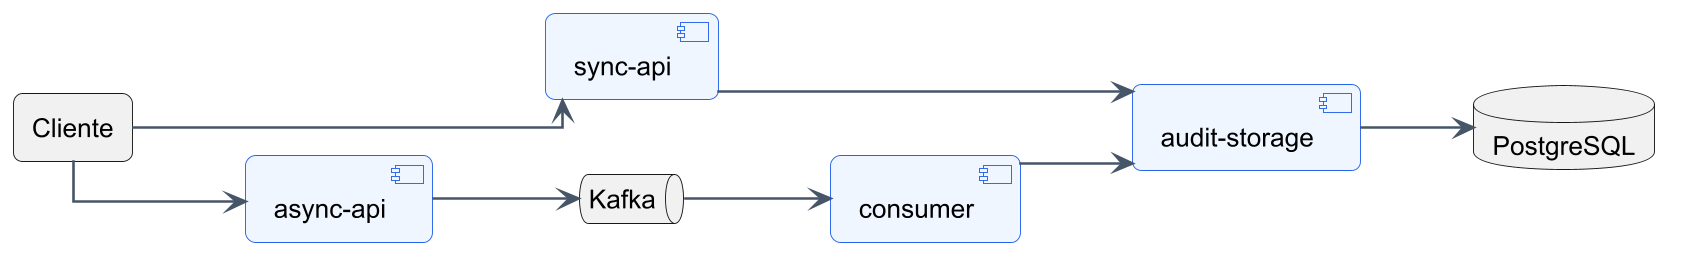
\includegraphics[width=0.95\textwidth,height=0.43\textheight,keepaspectratio]{Diagramas/plantuml/visao-geral.png}
\caption{Visão geral dos caminhos síncrono e assíncrono em Java}
\label{fig:visao-geral}
\fonte{Elaborado pelo autor (2026).}
\end{figure}

Nesta documentação, \textbf{implementado} indica que existe código para o comportamento descrito; as verificações disponíveis e seu alcance são apresentados na Seção~\ref{sec:validacao-funcional}. \textbf{Parcial} indica cobertura incompleta do requisito. \textbf{Planejado} identifica um componente ou procedimento ainda não implementado. Uma funcionalidade aprovada em teste não implica validação da hipótese científica.

A resposta \texttt{202 Accepted} sucede o ACK do broker e não significa que o registro já exista no PostgreSQL. Falhas de entrega podem produzir resultado incerto, enquanto falhas de consumo podem resultar em retry ou DLQ. A presença de uma mensagem na DLQ permite inspeção, mas não equivale a processamento concluído. O broker único limita a avaliação à topologia local, sem garantia de alta disponibilidade de cluster.

\textbf{Síntese.} As duas rotas executam o mesmo processamento e diferem na comunicação e nas condições de confirmação. O estado de cada requisito é vinculado ao código e às evidências, preservando a distinção entre validação funcional e comparação experimental.

\FloatBarrier
\section{Levantamento e especificação de requisitos}
\label{sec:requisitos}
Os identificadores RF01 a RF10 são preservados para manter a rastreabilidade com a documentação anterior. RF11 a RF15 tornam explícitas as funcionalidades de avaliação e interface previstas; RF16 e RF17 detalham tratamento de falhas e consulta por UUID. A prioridade \textbf{essencial} designa uma condição necessária ao núcleo ou à validade experimental; \textbf{desejável} designa uma facilidade de uso. A Tabela~\ref{tab:rf} distingue código Java existente de instrumentos planejados; o alcance dos testes está na Seção~\ref{sec:validacao-funcional}.

\subsection{Requisitos funcionais}
{\small
\begin{longtable}{>{\raggedright\arraybackslash}p{0.17\textwidth}>{\raggedright\arraybackslash}p{0.32\textwidth}>{\raggedright\arraybackslash}p{0.42\textwidth}}
\caption{Requisitos funcionais e critérios de aceitação}\label{tab:rf}\\
\hline
ID e estado & Descrição, prioridade e justificativa & Critério verificável de aceitação\\ \hline
\endfirsthead
\hline ID e estado & Descrição, prioridade e justificativa & Critério verificável de aceitação\\ \hline
\endhead
RF01\newline Implementado & Receber evento em \texttt{POST /audit}. Essencial: entrada equivalente nas variantes. & As duas APIs aceitam o mesmo JSON e retornam o UUID em respostas de sucesso.\\ \hline
RF02\newline Implementado & Validar contrato. Essencial: impedir dados estruturalmente inválidos. & UUID e data informados devem ser válidos; textos respeitam os limites do dicionário; entrada inválida retorna 422, sem processamento posterior.\\ \hline
RF03\newline Implementado & Concluir registro síncrono antes da resposta. Essencial: definir a semântica síncrona. & Resposta 201 ocorre somente após commit ou identificação de duplicata idêntica; status distingue \texttt{persisted} de \texttt{duplicate}.\\ \hline
RF04\newline Implementado & Encaminhar evento ao Kafka. Essencial: viabilizar processamento desacoplado. & Evento preserva UUID e conteúdo; chave é \texttt{entity\_id}. 202 somente após ACK individual do broker com tópico, partição e offset no log. Timeout de entrega retorna 503 com resultado incerto.\\ \hline
RF05\newline Implementado & Consumir mensagens. Essencial: concluir a rota assíncrona. & Mensagem válida do tópico configurado é desserializada, validada e encaminhada ao mesmo repositório da variante síncrona.\\ \hline
RF06\newline Implementado & Gerar hash determinístico. Essencial: detectar conteúdo divergente. & O mesmo evento completo gera o mesmo SHA-256 hexadecimal de 64 caracteres; a ordenação de chaves não altera a representação serializada.\\ \hline
RF07\newline Implementado & Persistir registro. Essencial: manter efeito observável. & Linha contém os campos de \texttt{AuditEvent} e \texttt{content\_hash}; \texttt{event\_id} é chave primária.\\ \hline
RF08\newline Implementado & Reconhecer reentrega idêntica. Essencial: evitar efeito duplicado. & Duas submissões com UUID e conteúdo iguais mantêm uma linha e retornam status de duplicata na segunda; conteúdo divergente não substitui o original.\\ \hline
RF09\newline Implementado & Confirmar offset após persistência. Essencial: reduzir risco de perda por confirmação antecipada. & Commit automático desativado; confirmar origem somente após persistência idempotente ou ACK da DLQ. Falha de confirmação mantém possibilidade de reentrega.\\ \hline
RF10\newline Implementado & Expor \texttt{GET /health}. Essencial: verificar resposta da API. & \texttt{/health} verifica PostgreSQL na API síncrona e metadados do tópico na assíncrona; retorna 200 ou 503. \texttt{/live} verifica apenas a resposta do processo.\\ \hline
RF11\newline Planejado & Coletar métricas por execução. Essencial: responder à pergunta experimental. & Um futuro coletor deverá produzir arquivos conciliáveis por UUID e execução, com aceitação, conclusão, throughput, erros e recursos, incluindo unidade e janela. Os logs Java isolados não satisfazem esse critério.\\ \hline
RF12\newline Parcial & Executar cenários de carga e falha. Essencial: controle experimental. & Há um \textit{smoke} de interrupção do banco na CI. O executor definitivo ainda deverá registrar taxa, duração, semente, variante, falha e configuração em manifesto reproduzível.\\ \hline
RF13\newline Parcial & Acompanhar recuperação. Essencial: avaliar comportamento após falhas. & O \textit{smoke} verifica retomada da saúde do banco, mas ainda falta registrar backlog, drenagem e conciliação dos eventos aceitos e persistidos.\\ \hline
RF14\newline Planejado & Consultar indicadores e comparar variantes. Desejável: facilitar inspeção. & Um relatório futuro deverá separar latência HTTP de conclusão e sinalizar ausência de dados. Não há interface ou normalizador comparativo Java implementado.\\ \hline
RF15\newline Planejado & Disponibilizar formulário de envio. Desejável: facilitar demonstração. & O wireframe preserva UUID e instante e distingue variantes. A interface dedicada e documentação interativa de API não integram a implementação Java atual.\\ \hline
RF16\newline Implementado & Tratar falhas e quarentena. Essencial: evitar perda por avanço prematuro. & Aplicar retry limitado com backoff; publicar erro terminal na DLQ e aguardar ACK antes de confirmar a origem.\\ \hline
RF17\newline Implementado & Consultar registro por UUID. Essencial: verificar efeito persistido. & A API síncrona retorna hash e timestamp da linha; 404 indica ausência observada e 503 indica consulta indisponível.\\ \hline
\end{longtable}
\noindent{\footnotesize Fonte: Elaborado pelo autor (2026).}\par
}

\subsection{Requisitos não funcionais}
A Tabela~\ref{tab:rnf} relaciona propriedades de qualidade, critérios verificáveis e justificativas.
Desempenho não é definido por um código HTTP: 201 e 202 não são limites de tempo. Não se impõe, antes do piloto, que a alternativa assíncrona seja mais rápida. Os critérios de medição e as condições de comparação substituem expressões não verificáveis como \textit{tempo reduzido}.

{\small
\begin{longtable}{>{\raggedright\arraybackslash}p{0.12\textwidth}>{\raggedright\arraybackslash}p{0.24\textwidth}>{\raggedright\arraybackslash}p{0.55\textwidth}}
\caption{Requisitos não funcionais}\label{tab:rnf}\\
\hline ID & Categoria e prioridade & Critério e justificativa\\ \hline
\endfirsthead
\hline ID & Categoria e prioridade & Critério e justificativa\\ \hline
\endhead
RNF01 & Equivalência; essencial & Utilizar DTO, serialização e repositório comuns; comparar o mesmo conjunto de eventos com a mesma configuração de persistência. Evita atribuir diferenças funcionais à comunicação.\\ \hline
RNF02 & Reprodutibilidade; essencial & Registrar imagens, dependências, commit, recursos, scripts e parâmetros. O Compose explicita limites de desenvolvimento; manifesto e checksums da coleta definitiva ainda precisam ser implementados e validados.\\ \hline
RNF03 & Segurança; essencial & Usar dados sintéticos sem segredos; executar em ambiente isolado. O protótipo não possui autenticação nem é autorizado para exposição pública ou dados pessoais reais.\\ \hline
RNF04 & Portabilidade; essencial & Descrever build e inicialização com Docker Compose, além dos pré-requisitos. Versões de bibliotecas são fixadas; tags de imagens deverão ter digest registrado na coleta.\\ \hline
RNF05 & Integridade e correlação; essencial & Preservar UUID e instante de origem nos reenvios; manter hash e restrição de unicidade. Conflitos devem ser distinguíveis de duplicatas legítimas nos registros de diagnóstico.\\ \hline
RNF06 & Desempenho; essencial & Medir latência de aceitação e de conclusão separadamente, p50/p95/p99, throughput persistido e taxa oferecida; definir tolerâncias de carga no piloto, conforme o Capítulo~\ref{cap:metodo}.\\ \hline
RNF07 & Resiliência; essencial & Após falha controlada e retomada, conciliar os UUIDs dentro da janela de drenagem; zero linhas duplicadas. Eventos na DLQ exigem tratamento posterior e não retornam automaticamente ao banco.\\ \hline
RNF08 & Observabilidade; essencial & Registrar execução, UUID, componente, etapa, instante e resultado; coletar recursos com intervalo fixado. Os marcos JSON já existem; coletores, completude e resolução temporal ainda precisam de validação para cada execução definitiva.\\ \hline
RNF09 & Escalabilidade; desejável & Registrar partições e número de consumidores em cada configuração. Não inferir escalabilidade horizontal a partir de uma execução em broker único.\\ \hline
RNF10 & Usabilidade experimental; desejável & Identificar a variante e o estado dos dados em cada tela; oferecer mensagens legíveis e unidades. Wireframes não equivalem a um painel implementado.\\ \hline
\end{longtable}
\noindent{\footnotesize Fonte: Elaborado pelo autor (2026).}\par
}

\subsection{Regras de negócio}
Neste contexto, regras de negócio são invariantes do processamento de auditoria e do contrato experimental, e não políticas de um sistema comercial.

\begin{description}
\item[RN01 --- Identidade.] Todo evento processado possui UUID. O DTO gera UUID se omitido; nos ensaios, o gerador deverá fornecê-lo antes do envio e preservá-lo nas novas tentativas. Novo UUID significa novo evento.
\item[RN02 --- Validação.] Tipo do evento, tipo e ID da entidade, ator e origem são obrigatórios e respeitam os limites do DTO. UUID, instante e payload possuem valores padrão quando omitidos. A obrigatoriedade no banco não significa obrigatoriedade de envio desses três campos na API. Na mensagem Kafka, identidade e instante devem estar explícitos: o consumidor rejeita sua ausência para que uma reentrega não gere outro evento.
\item[RN03 --- Hash.] O SHA-256 abrange todos os campos do evento validado, incluindo UUID e instante. JSON usa chaves ordenadas e separadores compactos. A regra é determinística no contexto da implementação; não se declara conformidade com um padrão externo de canonicalização.
\item[RN04 --- Idempotência.] Mesmo UUID e mesmo hash preservam a linha original e produzem status \texttt{duplicate}. O cliente deve reenviar o mesmo instante; gerar outra data pode tornar o conteúdo divergente.
\item[RN05 --- Conflito.] Mesmo UUID e hash diferente não podem sobrescrever a linha. A API síncrona retorna 409 com motivo \texttt{event\_id\_content\_conflict}. No consumidor, o conflito é encaminhado à DLQ sem alterar a linha original.
\item[RN06 --- Aceitação assíncrona.] O 202 não confirma persistência em PostgreSQL. Confirma publicação segundo \texttt{acks=all} e a topologia configurada. Se o ACK não chegar no prazo, a resposta 503 informa resultado incerto; o cliente deve conciliar e preservar o evento completo em eventual reenvio.
\item[RN07 --- Offset e falha.] O offset de origem é confirmado após inserção, reconhecimento idempotente ou ACK da DLQ. Falhas de persistência recebem tentativas limitadas com backoff. Se DLQ ou commit de offset não forem confirmados, a sessão é retomada sem avançar além da origem não resolvida.
\item[RN08 --- Confirmação síncrona.] A API retorna 201 após persistência ou reconhecimento de reentrega, distinguindo-os pelo campo status. Em falha de persistência não deve declarar sucesso.
\item[RN09 --- Particionamento.] A chave enviada ao produtor é \texttt{entity\_id}. A ordem relativa depende da manutenção da chave, do particionamento e da sequência produzida; não se promete ordenação global entre partições.
\item[RN10 --- Evidência experimental.] As métricas definitivas deverão identificar execução, variante, unidade e janela. Eventos gerados, aceitos e persistidos são conjuntos distintos. O marco pós-commit comum define conclusão; instante de ocorrência e timestamp de inserção não o substituem.
\item[RN11 --- Quarentena.] Mensagens inválidas, conflitos e tentativas esgotadas são retidos na DLQ. A chave de origem usa tópico, partição e offset. Se a DLQ for confirmada e o commit de origem falhar, podem existir cópias na DLQ; a conciliação futura deverá usar essa chave. Não há replay automático de mensagens em quarentena.
\end{description}
\textbf{Síntese.} Os requisitos indicam o comportamento esperado, o critério de verificação e o estado de implementação. As regras tornam explícitos os limites do aceite assíncrono, da identidade do evento e da recuperação.

\section{Modelagem UML}
\label{sec:uml}
As vistas representam o contrato, as responsabilidades e os caminhos de execução. A fronteira operacional é a implementação Java, com duas APIs Spring Boot e um consumidor independente; Kafka e PostgreSQL são sistemas externos de suporte. Na visão de implantação, esses serviços integram a infraestrutura do ambiente experimental. As bibliotecas Maven compartilhadas não são atores nem processos independentes.

\subsection{Diagrama de casos de uso}
A aplicação cliente inicia UC01 e UC02; Kafka fornece mensagens a UC03; o pesquisador consulta prontidão e registros em UC04 e UC07. A Figura~\ref{fig:casos-uso} apresenta essas interações. A Figura~\ref{fig:casos-exp} reúne os casos planejados de avaliação quantitativa, cujo executor ainda não integra o projeto Java.

\capfig{casos-de-uso}{Casos de uso da aplicação operacional}{fig:casos-uso}{0.44}
\capfig{casos-experimento}{Casos de uso da camada de avaliação}{fig:casos-exp}{0.25}

\subsubsection{UC01 --- Registrar auditoria sincronamente}
\textbf{Objetivo e atores:} persistir evento antes da resposta; aplicação cliente e PostgreSQL.
\textbf{Pré-condições:} API inicializada e banco acessível.
\textbf{Ativação:} \texttt{POST /audit}.
\textbf{Pós-condição:} linha inserida ou reentrega idêntica reconhecida.
\textbf{Regras:} RN01--RN05 e RN08.
\begin{enumerate}
\item A aplicação envia o evento à API síncrona.
\item O contrato é validado e recebe os valores padrão permitidos.
\item O repositório calcula a representação determinística e o SHA-256.
\item Executa \texttt{INSERT ON CONFLICT DO NOTHING}, verificando o resultado.
\item A transação é concluída; o marco pós-commit é registrado.
\item A API retorna 201, UUID, hash, status e timestamp de inserção.
\end{enumerate}
\textbf{A1 --- Reentrega:} quando o UUID já existe, uma nova consulta na mesma transação em \texttt{READ COMMITTED} obtém a linha. Hash igual produz \texttt{duplicate}; nenhuma nova linha é criada.
\textbf{E1 --- Contrato inválido:} retorna 422 antes de chamar o repositório.
\textbf{E2 --- Conflito:} hash diferente provoca rollback e resposta 409 com \texttt{event\_id\_content\_conflict}, preservando a linha original.
\textbf{E3 --- Banco indisponível:} retorna 503 com \texttt{database\_unavailable}. Uma falha durante o commit pode deixar o resultado incerto; consulta e reenvio devem preservar o evento completo.

\subsubsection{UC02 --- Aceitar auditoria assincronamente}
\textbf{Objetivo e atores:} confirmar publicação sem aguardar persistência; aplicação cliente e Kafka.
\textbf{Pré-condição:} API e publicador inicializados.
\textbf{Ativação:} \texttt{POST /audit} na API assíncrona.
\textbf{Pós-condição:} publicação confirmada individualmente pelo broker.
\textbf{Regras:} RN01, RN02, RN06 e RN09.
\begin{enumerate}
\item A API valida o mesmo contrato da variante síncrona.
\item Serializa os campos completos e usa \texttt{entity\_id} como chave.
\item O publicador chama \texttt{send(...).get(...)} e aguarda a confirmação individual dentro do prazo.
\item Registra o ACK, incluindo tópico, partição e offset, e retorna 202.
\end{enumerate}
\textbf{A1 --- Reenvio:} a API não consulta duplicidade; o consumidor e o banco reconhecem eventos idênticos.
\textbf{E1 --- Contrato inválido:} retorna 422.
\textbf{E2 --- Buffer do produtor cheio:} retorna 503 com \texttt{acceptance=rejected}.
\textbf{E3 --- Timeout ou erro de confirmação:} retorna 503 com \texttt{acceptance=unknown}. A mensagem pode ter sido entregue; a resposta não autoriza assumir perda.
\textbf{Limite:} ACK de publicação e persistência são pós-condições distintas. O consumidor pode processar a mensagem antes ou depois de o cliente receber a resposta.

\subsubsection{UC03 --- Consumir e persistir evento}
\textbf{Objetivo e atores:} processar ou reter uma falha identificável; Kafka e PostgreSQL.
\textbf{Pré-condições:} consumidor inscrito no tópico e configuração de retry válida.
\textbf{Ativação:} mensagem retornada por \texttt{poll}.
\textbf{Pós-condição:} persistência idempotente ou retenção confirmada na DLQ, seguida da confirmação da posição de origem.
\textbf{Regras:} RN03--RN05, RN07, RN09 e RN11.
\begin{enumerate}
\item O consumidor recebe a mensagem e recupera o identificador da execução.
\item Valida JSON, contrato e presença explícita de UUID e instante.
\item Registra a tentativa e chama o repositório comum.
\item Depois da transação ou reconhecimento de duplicata, registra o resultado.
\item Confirma o offset de origem de forma síncrona e retorna à espera.
\end{enumerate}
\textbf{A1 --- Reentrega idêntica:} preserva a linha e confirma a posição após reconhecimento de duplicata.
\textbf{A2 --- Falha transitória:} repete a persistência até o limite configurado, com backoff exponencial limitado e registro das tentativas.
\textbf{E1 --- Mensagem inválida, conflito ou tentativas esgotadas:} publica envelope na DLQ com identidade da origem, motivo e conteúdo original, aguarda ACK e então confirma a origem.
\textbf{E2 --- DLQ não confirmada:} retoma a sessão sem confirmar a mensagem de origem. Mensagens posteriores não justificam avançar sua posição.
\textbf{E3 --- Falha de commit de offset:} retoma a sessão; a persistência ou a publicação em DLQ já pode ter ocorrido. A reentrega é tratada por UUID no banco ou pela identidade da origem na conciliação da DLQ.
\textbf{E4 --- Dependência indisponível:} o laço externo aguarda e reinicia a sessão; a política de restart do Compose cobre encerramento do processo. Mensagens já retidas na DLQ exigem inspeção e não retornam automaticamente ao fluxo principal.

\subsubsection{UC04 --- Consultar prontidão}
\textbf{Ator:} pesquisador.
\textbf{Ativação:} \texttt{GET /health}.
\textbf{Pré-condição:} processo HTTP iniciado.
\textbf{Fluxo principal:} verificar acesso ao esquema PostgreSQL na API síncrona ou existência e liderança das partições do tópico na API assíncrona; retornar 200 com \texttt{ready}.
\textbf{Alternativa:} \texttt{GET /live} retorna \texttt{alive} para verificar apenas a resposta do processo.
\textbf{Exceção:} dependência sem prontidão produz 503; processo parado causa falha de conexão.
\textbf{Pós-condição:} resultado de uma verificação pontual, sem garantia de disponibilidade futura ou de conclusão de todos os eventos. Relaciona-se a RF10.

\subsubsection{UC05 --- Executar cenário de avaliação (planejado)}
\textbf{Ator:} pesquisador.
\textbf{Pré-condições:} ambiente isolado preparado, dados sintéticos e configuração identificada; protocolo congelado para coleta definitiva.
\textbf{Ativação prevista:} comando do executor e seleção do perfil.
\textbf{Fluxo previsto:} criar diretório exclusivo; registrar manifesto; preparar eventos; executar aquecimento e carga; coletar logs, recursos e offsets; interromper o PostgreSQL em C4; registrar a retomada; aguardar drenagem; consolidar arquivos.
\textbf{Alternativas:} teste dos instrumentos ou execução conforme protocolo definitivo.
\textbf{Exceção prevista:} configuração incompleta ou falha de coleta deve ser registrada; validação funcional não vira resultado definitivo.
\textbf{Pós-condição esperada:} artefatos verificáveis da execução, com indicação de completude. O projeto Java atual contém apenas \textit{smokes} de CI, sem esse executor. Relaciona-se a RF12, RF13 e RN10.

\subsubsection{UC06 --- Consolidar e consultar indicadores (planejado)}
\textbf{Ator:} pesquisador.
\textbf{Pré-condição:} arquivos brutos de execução disponíveis.
\textbf{Ativação prevista:} execução de um normalizador ainda não adaptado ao Java.
\textbf{Fluxo previsto:} verificar arquivos; correlacionar UUIDs; separar fases; calcular métricas e unidades; registrar inconsistências; produzir tabelas e relatório.
\textbf{Alternativa:} inspecionar lag, reentregas, retry, DLQ e recuperação.
\textbf{Exceção:} ausência de instrumentação é sinalizada e não substituída por medição zero.
\textbf{Pós-condição esperada:} indicadores rastreáveis aos dados brutos. A interface dedicada dos wireframes permanece proposta. Relaciona-se a RF11, RF14 e RN10.

\subsubsection{UC07 --- Consultar registro por UUID}
\textbf{Ator:} pesquisador ou aplicação cliente.
\textbf{Pré-condições:} API síncrona e banco acessíveis.
\textbf{Ativação:} \texttt{GET /audit/\{event\_id\}}.
\textbf{Fluxo principal:} validar UUID, consultar a projeção da linha e retornar 200 com hash e timestamp.
\textbf{Alternativa:} após reenvio, conferir a preservação do hash.
\textbf{Exceções:} UUID inválido retorna 422; linha não localizada, 404; banco indisponível, 503.
\textbf{Pós-condição:} existência ou ausência observada naquele instante; 404 durante processamento assíncrono não prova perda. Relaciona-se a RF17 e RN04.

\subsection{Diagramas de atividades}
A Figura~\ref{fig:atividade-sync} representa a inserção síncrona e as decisões de duplicidade e conflito. As Figuras~\ref{fig:atividade-async} e~\ref{fig:atividade-consumidor} separam o aceite da API produtora e o processamento do consumidor. Os dois processos assíncronos não dependem da ordem em que a resposta HTTP chega ao cliente.

\capfig{atividade-sincrona}{Atividade síncrona: transação, duplicidade e conflito}{fig:atividade-sync}{0.62}
\capfig{atividade-assincrona}{Atividade da API produtora e confirmação de publicação}{fig:atividade-async}{0.59}
\capfig{atividade-consumidor}{Atividade do consumidor, retry e confirmação da origem}{fig:atividade-consumidor}{0.75}

A atividade de persistência com retry corresponde ao laço limitado de UC03. O caminho de quarentena inclui a espera pelo ACK da DLQ. Um término da iteração não significa encerramento do serviço: o laço externo mantém a espera ou a reconexão, conforme indicado nas ações.

\FloatBarrier
\subsection{Diagramas de classes}
A Figura~\ref{fig:classes-dados} apresenta os \textit{records} do contrato e o repositório JDBC. A Figura~\ref{fig:classes} mostra as classes de entrada e processamento dos três módulos executáveis, além das dependências compartilhadas. Nenhuma herança ORM é representada porque o projeto Java usa Spring JDBC e uma migração SQL.

\capfig{classes-dados}{Classes de contrato e persistência}{fig:classes-dados}{0.46}
\capfig{classes}{Classes de aplicação e processamento Java}{fig:classes}{0.45}

A notação \(+\) indica membros públicos. A validação pertence ao contrato \texttt{AuditEvent}. A serialização e o hash ficam na \texttt{CanonicalEventCodec}; a transação, na \texttt{AuditRepository}; e os marcos, na \texttt{MilestoneLog}. O broker é infraestrutura, não classe de domínio. O \texttt{AuditMessageProcessor} chama \texttt{commitSync} sobre o consumidor Kafka depois da persistência ou do ACK da DLQ.

\FloatBarrier
\subsection{Diagramas complementares}
As Figuras~\ref{fig:seq-sync} e~\ref{fig:seq-async} detalham a ordem entre transação, resposta, ACK e confirmação de posição. A Figura~\ref{fig:componentes} sintetiza as dependências entre os módulos Maven; o caminho de publicação na DLQ pelo consumidor é detalhado na atividade, na sequência e na arquitetura assíncronas para manter esta vista legível. As Figuras~\ref{fig:arq-sync} e~\ref{fig:arq-async} distinguem os fluxos arquiteturais e a participação da DLQ.

\capfig{sequencia-sincrona}{Sequência síncrona com inserção idempotente}{fig:seq-sync}{0.62}
\capfig{sequencia-assincrona}{Sequência assíncrona com ACK e tratamento de falhas}{fig:seq-async}{0.61}
\capfig{componentes}{Dependências entre os cinco módulos Maven}{fig:componentes}{0.44}
\capfig{arquitetura-sincrona}{Arquitetura da variante síncrona}{fig:arq-sync}{0.38}
\capfig{arquitetura-assincrona}{Arquitetura da variante assíncrona e DLQ}{fig:arq-async}{0.43}

\subsubsection{Diagrama de implantação}
A Figura~\ref{fig:implantacao} localiza os cinco serviços permanentes na rede Docker Compose e separa o cliente de carga, executado pelo pesquisador, dos processos de aplicação. Os serviços \texttt{kafka-init} e \texttt{kafka-volume-init} são transitórios e, por isso, aparecem na anotação do diagrama, não como processos permanentes. As portas publicadas estão restritas ao \textit{loopback} do host. Os volumes nomeados conservam os dados do PostgreSQL e os logs do Kafka entre reinícios de contêiner. Esta é uma implantação experimental com um broker, uma partição por tópico e um banco; não representa alta disponibilidade.

\capfig{implantacao}{Implantação real do protótipo no Docker Compose}{fig:implantacao}{0.48}

\FloatBarrier
\subsection{Rastreabilidade entre requisitos, regras e UML}
A Tabela~\ref{tab:rastreabilidade} relaciona cada requisito funcional às regras e aos elementos que o representam. Os elementos planejados não indicam código já existente. A cobertura funcional verificada é delimitada na Seção~\ref{sec:validacao-funcional}.
{\small
\begin{longtable}{p{0.20\textwidth}p{0.20\textwidth}p{0.51\textwidth}}
\caption{Rastreabilidade funcional e comportamental}\label{tab:rastreabilidade}\\
\hline Requisitos & Regras & Casos e elementos de modelagem\\ \hline
\endfirsthead
\hline Requisitos & Regras & Casos e elementos de modelagem\\ \hline
\endhead
RF01, RF02 & RN01, RN02 & UC01, UC02; AuditEvent e validação dos dois fluxos.\\ \hline
RF03, RF06, RF07 & RN03, RN08 & UC01; atividade e sequência síncronas; CanonicalEventCodec e AuditRepository.\\ \hline
RF04 & RN06, RN09 & UC02; KafkaPublisher; ACK na atividade e sequência assíncronas.\\ \hline
RF05, RF09, RF16 & RN07, RN11 & UC03; retry, DLQ e confirmação de origem; atividade do consumidor.\\ \hline
RF08 & RN04, RN05 & UC01 e UC03; decisões de hash e unicidade; tabela audit\_records.\\ \hline
RF10 & RN10 & UC04; prontidão e vivacidade das APIs.\\ \hline
RF11, RF14 & RN10 & UC06 planejado; normalizador e wireframes de métricas/comparação.\\ \hline
RF12, RF13 & RN07, RN10 & UC05 planejado; protocolo e acompanhamento de backlog ainda incompletos.\\ \hline
RF15 & RN01, RN02, RN06 & UC01 e UC02; wireframe de envio com identidade preservada.\\ \hline
RF17 & RN04, RN05 & UC07; consulta por UUID no repositório.\\ \hline
\end{longtable}
\noindent{\footnotesize Fonte: Elaborado pelo autor (2026).}\par
}
\textbf{Síntese.} Os casos de uso descrevem objetivos e exceções; atividades e sequências mostram as decisões; classes e componentes localizam suas responsabilidades. As condições da coleta definitiva permanecem ligadas ao protocolo metodológico.

\section{Modelagem de banco de dados}
\label{sec:banco}
A modelagem distingue o esquema operacional da extensão relacional proposta. O banco da implementação Java possui somente a tabela \texttt{audit\_records}, criada pela migração Flyway \texttt{V1\_\_create\_audit\_records.sql}. O acesso usa Spring JDBC; não há mapeamento ORM nem rotina de adaptação de linhas históricas da versão Python. Marcos de execução são emitidos nos logs da aplicação, fora do banco operacional. A coleta estruturada de métricas e tentativas para o experimento ainda será desenvolvida. As tabelas adicionais desta seção permanecem propostas opcionais.

\subsection{Modelo conceitual (MER)}
A Figura~\ref{fig:mer-atual} apresenta o núcleo e a Figura~\ref{fig:mer-proposto} apresenta a extensão proposta. No núcleo atual, a entidade \textit{Registro de auditoria} representa o fato persistido e contém identificação, origem, instante, entidade, ator, conteúdo e hash. Não há relacionamento entre tabelas no esquema existente. O hash é atributo do registro, pois há exatamente um digest armazenado por linha; criar uma entidade \textit{EventHash} independente não acrescentaria informação necessária ao recorte e criaria uma sincronização adicional.

A extensão proposta introduz \textit{Log de processamento}, \textit{Tentativa de recuperação} e \textit{Amostra de métrica}. Um UUID pode aparecer em zero ou muitos logs, inclusive quando nenhuma linha de auditoria foi persistida. Cada log representa uma tentativa ou etapa observada. Um log pode originar zero ou muitas tentativas de recuperação; cada tentativa referencia um log. Métricas agregadas são associadas ao identificador da execução, e não obrigatoriamente a um único evento.

\capfig{mer-atual}{Modelo conceitual do núcleo existente}{fig:mer-atual}{0.25}
\capfig{mer-proposto}{Modelo conceitual da extensão de observabilidade proposta}{fig:mer-proposto}{0.40}

A associação entre registro e log é de correlação por UUID, não de existência obrigatória: um erro pode ocorrer antes da primeira inserção. Não se estabelece uma chave estrangeira obrigatória de log para \texttt{audit\_records}, pois isso impediria registrar justamente a falha de persistência. A tentativa de recuperação, por sua vez, referencia um log já existente. Essa distinção preserva a capacidade de registrar eventos rejeitados, falhas e reentregas sem pressupor sucesso.

\subsection{Modelo lógico}
No esquema atual, \texttt{audit\_records.event\_id} é chave primária; \texttt{entity\_id} possui o índice secundário \texttt{idx\_audit\_records\_entity\_id}; os atributos do evento e o hash são não nulos. A coluna \texttt{persisted\_at} é anulável no DDL, embora novas inserções recebam \texttt{clock\_timestamp()} por padrão. A Figura~\ref{fig:der-atual} representa somente a tabela implementada. Não existem chaves estrangeiras ou relacionamentos entre tabelas. A restrição de unicidade protege contra inserções concorrentes com o mesmo UUID. O hash é calculado na aplicação e armazenado como texto; não há restrição SQL de comprimento do digest.

\capfig{modelo-logico-atual}{Modelo lógico do banco implementado}{fig:der-atual}{0.38}

\subsection{Modelo físico implementado}
O arquivo \texttt{audit-storage/src/main/resources/db/migration/V1\_\_create\_audit\_records.sql} cria a tabela no PostgreSQL. Sua chave primária sobre \texttt{event\_id} é a única restrição de unicidade explícita. \texttt{entity\_id} recebe índice não único \texttt{idx\_audit\_records\_entity\_id}. Os nove campos obrigatórios são \texttt{event\_id}, \texttt{event\_type}, \texttt{entity\_type}, \texttt{entity\_id}, \texttt{actor\_id}, \texttt{source}, \texttt{occurred\_at}, \texttt{payload} e \texttt{content\_hash}. O décimo campo, \texttt{persisted\_at}, é anulável e possui \texttt{DEFAULT clock\_timestamp()}. Não existe chave estrangeira, gatilho, exclusão lógica ou tabela de usuários nesse esquema.

O Flyway aplica a migração V1 na inicialização da API síncrona e do consumidor sobre o banco novo desta versão. Não há migração automática do banco Python nem compatibilidade retroativa demonstrada. A garantia de idempotência combina a PK, o \texttt{INSERT ON CONFLICT DO NOTHING} e a comparação do \texttt{content\_hash} no \texttt{AuditRepository} após a tentativa de inserção. Portanto, o modelo físico deve ser entendido junto à regra implementada na aplicação, e não como uma restrição SQL de igualdade do conteúdo.

\subsection{Extensão lógica opcional}
A Figura~\ref{fig:der} apresenta, separadamente, a possível extensão de observabilidade. As entidades destacadas como \textit{propostas} não foram criadas pelo código e não integram o banco utilizado nos testes.

\capfig{modelo-logico}{Modelo lógico da extensão proposta, separado do esquema atual}{fig:der}{0.57}

Na extensão, \texttt{processing\_log.id}, \texttt{retry\_log.id} e \texttt{metrics.id} são chaves primárias propostas. \texttt{retry\_log.processing\_log\_id} referencia o log que motivou a tentativa. \texttt{run\_id} correlaciona os três conjuntos com o manifesto externo de execução. Não se cria uma tabela de execuções nesta proposta inicial; caso isso seja feito posteriormente, o manifesto poderá ser normalizado em uma entidade própria.

A unicidade proposta de \texttt{(run\_id, event\_id, component, attempt)} em logs identifica uma tentativa por componente. Índices por execução, UUID e instante apoiam conciliação. Status e unidades deverão ser validados pela camada de coleta. Migrações e consultas dessas tabelas são atividades futuras, não executadas para produzir este texto. A instrumentação deverá ser equivalente entre variantes e ter seu custo considerado na análise experimental.

\FloatBarrier
\subsection{Dicionário de dados}

\subsubsection{Tabela audit\_records --- existente}
A Tabela~\ref{tab:dic-audit} descreve o esquema efetivo. Os campos do evento e o hash são não nulos; \texttt{persisted\_at} admite nulo pelo DDL da migração Java. No recebimento HTTP, \texttt{event\_id}, \texttt{occurred\_at} e \texttt{payload} podem ser omitidos e recebem valores padrão.

{\small
\begin{longtable}{>{\raggedright\arraybackslash}p{0.23\textwidth}>{\raggedright\arraybackslash}p{0.22\textwidth}>{\raggedright\arraybackslash}p{0.46\textwidth}}
\caption{Dicionário do registro persistido}\label{tab:dic-audit}\\
\hline Campo & Tipo e tamanho & Obrigatoriedade, significado e validação\\ \hline
\endfirsthead
\hline Campo & Tipo e tamanho & Obrigatoriedade, significado e validação\\ \hline
\endhead
\texttt{event\_id} & UUID, 128 bits & PK; não nulo. UUID informado deve ser válido; uuid4 gerado se ausente. Deve ser preservado em reenvios experimentais.\\ \hline
\texttt{event\_type} & VARCHAR(100) & Não nulo; obrigatório na API, 1--100 caracteres. Tipo do fato observado; sem enumeração fechada implementada.\\ \hline
\texttt{entity\_type} & VARCHAR(100) & Não nulo; obrigatório, 1--100 caracteres. Tipo da entidade referida.\\ \hline
\texttt{entity\_id} & VARCHAR(200) & Não nulo; obrigatório, 1--200 caracteres; índice. Identificador da entidade e chave enviada ao Kafka.\\ \hline
\texttt{actor\_id} & VARCHAR(200) & Não nulo; obrigatório, 1--200 caracteres. Ator sintético relacionado ao fato.\\ \hline
\texttt{source} & VARCHAR(100) & Não nulo; obrigatório, 1--100 caracteres. Sistema ou componente de origem.\\ \hline
\texttt{occurred\_at} & TIMESTAMP WITH TIME ZONE & Não nulo. Instante de ocorrência; padrão UTC atual se omitido. Quando informado, o Java interpreta data ISO-8601 com offset. Não representa instante de commit.\\ \hline
\texttt{payload} & JSONB & Não nulo; objeto com padrão vazio. Sem limite de tamanho ou profundidade definido no DTO atual. Conteúdo contextual sintético.\\ \hline
\texttt{content\_hash} & TEXT & Não nulo. SHA-256 calculado, 64 caracteres hexadecimais; o tipo SQL não impõe esse comprimento. Inclui os campos completos do evento.\\ \hline
\texttt{persisted\_at} & TIMESTAMP WITH TIME ZONE & Anulável pelo DDL. Novas linhas recebem clock\_timestamp() durante INSERT. Não representa conclusão do commit.\\ \hline
\end{longtable}
\noindent{\footnotesize Fonte: Elaborado pelo autor (2026).}\par
}

\subsubsection{Tabela processing\_log --- proposta}
A Tabela~\ref{tab:dic-processing} descreve a proposta de uma tentativa por componente. Ela não substitui o evento original nem modifica sua identidade.

{\small
\begin{longtable}{>{\raggedright\arraybackslash}p{0.23\textwidth}>{\raggedright\arraybackslash}p{0.22\textwidth}>{\raggedright\arraybackslash}p{0.46\textwidth}}
\caption{Dicionário proposto dos logs de processamento}\label{tab:dic-processing}\\
\hline Campo & Tipo e tamanho & Obrigatoriedade e regra proposta\\ \hline
\endfirsthead
\hline Campo & Tipo e tamanho & Obrigatoriedade e regra proposta\\ \hline
\endhead
\texttt{id} & BIGINT identity & PK, obrigatório. Identifica o log.\\ \hline
\texttt{run\_id} & UUID & Obrigatório. Correlaciona com o manifesto de execução.\\ \hline
\texttt{event\_id} & UUID & Obrigatório para eventos identificáveis. Correlação, sem FK para o registro persistido. Erros sem UUID ficam no log técnico do coletor.\\ \hline
\texttt{component} & VARCHAR(30) & Obrigatório. Identifica API síncrona, API produtora ou consumidor.\\ \hline
\texttt{status} & VARCHAR(30) & Obrigatório. Vocabulário proposto: accepted, persisted, duplicate, rejected, failed ou conflict.\\ \hline
\texttt{attempt} & INTEGER & Obrigatório; maior ou igual a 1. Número da tentativa por evento e componente na execução.\\ \hline
\texttt{started\_at} & TIMESTAMPTZ & Obrigatório. Início da tentativa em UTC.\\ \hline
\texttt{finished\_at} & TIMESTAMPTZ & Opcional enquanto a tentativa estiver aberta; ao concluir, não anterior ao início.\\ \hline
\texttt{detail} & TEXT & Opcional. Diagnóstico sem credenciais ou conteúdo sensível.\\ \hline
\end{longtable}
\noindent{\footnotesize Fonte: Elaborado pelo autor (2026).}\par
}

\subsubsection{Tabela retry\_log --- proposta}
A Tabela~\ref{tab:dic-retry} descreve os campos da extensão para recuperação.
{\small
\begin{longtable}{>{\raggedright\arraybackslash}p{0.23\textwidth}>{\raggedright\arraybackslash}p{0.22\textwidth}>{\raggedright\arraybackslash}p{0.46\textwidth}}
\caption{Dicionário proposto das tentativas de recuperação}\label{tab:dic-retry}\\
\hline Campo & Tipo e tamanho & Obrigatoriedade e regra proposta\\ \hline
\endfirsthead
\hline Campo & Tipo e tamanho & Obrigatoriedade e regra proposta\\ \hline
\endhead
\texttt{id} & BIGINT identity & PK, obrigatório.\\ \hline
\texttt{processing\_log\_id} & BIGINT & FK obrigatória para processing\_log.id; identifica a tentativa anterior relacionada.\\ \hline
\texttt{reason} & VARCHAR(200) & Obrigatório. Motivo da retomada, sem dados sensíveis.\\ \hline
\texttt{retried\_at} & TIMESTAMPTZ & Obrigatório. Instante da nova tentativa; não apenas um agendamento futuro.\\ \hline
\end{longtable}
\noindent{\footnotesize Fonte: Elaborado pelo autor (2026).}\par
}
O vínculo proposto ao log fornece execução, UUID e componente sem replicar esses campos. A política automática de retry está implementada no consumidor e emite marcos JSON no fluxo de logs; sua existência não depende da criação desta tabela.

\subsubsection{Tabela metrics --- proposta}
A Tabela~\ref{tab:dic-metrics} descreve uma possível persistência relacional das métricas a serem coletadas no experimento Java.
{\small
\begin{longtable}{>{\raggedright\arraybackslash}p{0.23\textwidth}>{\raggedright\arraybackslash}p{0.22\textwidth}>{\raggedright\arraybackslash}p{0.46\textwidth}}
\caption{Dicionário proposto das amostras de métricas}\label{tab:dic-metrics}\\
\hline Campo & Tipo e tamanho & Obrigatoriedade e regra proposta\\ \hline
\endfirsthead
\hline Campo & Tipo e tamanho & Obrigatoriedade e regra proposta\\ \hline
\endhead
\texttt{id} & BIGINT identity & PK, obrigatório.\\ \hline
\texttt{run\_id} & UUID & Obrigatório. Correlaciona com o manifesto.\\ \hline
\texttt{variant} & VARCHAR(10) & Obrigatório: sync ou async.\\ \hline
\texttt{metric\_type} & VARCHAR(50) & Obrigatório. Identifica latência, throughput, erro, recurso ou backlog.\\ \hline
\texttt{value} & DOUBLE PRECISION & Obrigatório; valor finito. Ausência de amostra não deve ser registrada como zero.\\ \hline
\texttt{unit} & VARCHAR(20) & Obrigatório. Unidade explícita, como ms, eventos/s, bytes ou percentual.\\ \hline
\texttt{window\_start} & TIMESTAMPTZ & Obrigatório. Início da janela de medição.\\ \hline
\texttt{window\_end} & TIMESTAMPTZ & Obrigatório; igual ou posterior ao início.\\ \hline
\end{longtable}
\noindent{\footnotesize Fonte: Elaborado pelo autor (2026).}\par
}

A medição de conclusão utiliza o marco \texttt{commit\_completed} emitido após a transação. Nem \texttt{occurred\_at} nem \texttt{persisted\_at} substituem esse marco. Consultas periódicas oferecem uma observação posterior da linha, sujeita ao intervalo de consulta, à duração da requisição e ao escalonamento; portanto, o intervalo configurado sozinho não estabelece um limite rígido para todo o atraso de observação.

\textbf{Síntese.} O esquema existente garante unicidade e conserva conteúdo e hash. O modelo proposto amplia a rastreabilidade de falhas e métricas sem impor uma FK que impeça registrar tentativas fracassadas e sem apresentar essas tabelas como já implementadas.

\section{Prototipação da interface}
\label{sec:interface}
O núcleo atual é uma API, sem frontend próprio. Os wireframes desta seção representam interfaces propostas de operação e inspeção, não capturas de telas funcionais. As telas não executam o experimento nem contêm resultados medidos; usam estados vazios para indicar o que deverá ser apresentado após instrumentação.

\subsection{Envio de registro}
A Figura~\ref{fig:wf-envio} apresenta WF01, que permite escolher a variante e informar todos os campos do contrato. O usuário poderá gerar UUID e instante antes do envio e reutilizá-los em uma reentrega. A ação de envio mostrará código HTTP, corpo da resposta e UUID. Na variante assíncrona, a interface deverá distinguir aceitação de conclusão e não apresentar 202 como comprovante de persistência. Os campos obrigatórios e seus limites seguem o dicionário da Seção~\ref{sec:banco}. Relaciona-se a RF01, RF02 e RF15.
\capfig{wf-envio}{WF01: wireframe proposto para envio de registros}{fig:wf-envio}{0.39}

\subsection{Visualização de métricas}
A Figura~\ref{fig:wf-metricas} apresenta WF02, que seleciona execução, variante e janela; apresenta taxa oferecida, throughput persistido, erros e percentis. Aceitação e conclusão ficam em campos distintos. O botão de exportação representa integração futura com os arquivos que serão produzidos pelo executor experimental Java. Falta de instrumentação deve aparecer como ausência de dados, não como medição igual a zero. Relaciona-se a RF11 e RF14.
\capfig{wf-metricas}{WF02: wireframe proposto para métricas}{fig:wf-metricas}{0.32}

\subsection{Acompanhamento de backlog}
A Figura~\ref{fig:wf-backlog} apresenta WF03, que permite inspecionar tópico, grupo e estado de coleta. Exibe offsets, diferença de posições e quantidade conciliada de eventos aceitos e persistidos. Esses números não são intercambiáveis: offsets dependem de partições e confirmações, enquanto a conciliação depende de UUIDs. O controle de falhas deverá exigir identificação do cenário e registrar os instantes de interrupção e retomada. Relaciona-se a RF12 e RF13.
\capfig{wf-backlog}{WF03: wireframe proposto para backlog e recuperação}{fig:wf-backlog}{0.34}

\subsection{Comparação entre variantes}
A Figura~\ref{fig:wf-comparacao} apresenta WF04, que organiza lado a lado as mesmas métricas por variante. A interface deverá impedir comparação entre configurações incompatíveis ou apresentar explicitamente as diferenças. A latência de aceitação não substituirá a de conclusão. Não haverá rótulo de vencedor automático: a interpretação considera dispersão, recursos, falhas e limites de generalização. Relaciona-se a RF14 e RN10.
\capfig{wf-comparacao}{WF04: wireframe proposto para comparação experimental}{fig:wf-comparacao}{0.32}

\textbf{Síntese.} Os quatro wireframes descrevem a interação desejada e os estados sem dados. A interface dedicada permanece proposta; os \textit{smokes} e testes Java descritos na Seção~\ref{sec:validacao-funcional} fornecem evidência funcional limitada, mas ainda não alimentam essas telas. As imagens desta seção representam exclusivamente prototipação de interface.

\section{Implementação do sistema}
\label{sec:implementacao-real}
Esta versão do protótipo foi implementada em Java e inspecionada em 29 de setembro de 2026. O projeto é uma implementação paralela do mesmo recorte experimental, não uma comparação entre linguagens. O código-fonte e sua configuração estão no repositório \url{https://github.com/ilann47/TCC-2026}, no diretório \texttt{implementacao-java}. As verificações funcionais descritas nesta seção não constituem a coleta quantitativa definitiva prevista no Capítulo~\ref{cap:metodo}.

\subsection{Tecnologias e módulos}
O projeto utiliza Java com bytecode alvo 21, Spring Boot 3.5.16, Maven Wrapper, driver PostgreSQL, Spring JDBC, Flyway, cliente Apache Kafka 3.9.1 e springdoc-openapi 2.9.1 para a documentação das APIs. A implantação descrita em \texttt{docker-compose.yml} utiliza PostgreSQL 16 e Kafka 3.9.1. O Maven compila cinco módulos: \texttt{audit-core}, \texttt{audit-storage}, \texttt{sync-api}, \texttt{async-api} e \texttt{consumer}. Os dois primeiros são bibliotecas compartilhadas; os três últimos são processos executáveis independentes.

\begin{table}[htbp]
\centering\small
\caption{Módulos Java e responsabilidades efetivas}\label{tab:modulos-implementados}
\begin{tabular}{p{0.24\textwidth}p{0.65\textwidth}}
\hline
Módulo & Responsabilidade\\ \hline
\texttt{audit-core} & Contrato \texttt{AuditEvent}, serialização determinística, SHA-256, publicação Kafka e marcos de observabilidade.\\
\texttt{audit-storage} & Migração Flyway V1, transação JDBC, consulta, comparação de hash e persistência idempotente.\\
\texttt{sync-api} & \texttt{POST /audit}, \texttt{GET /audit/\{event\_id\}}, \texttt{/live} e \texttt{/health}; grava antes da resposta 201.\\
\texttt{async-api} & \texttt{POST /audit}, \texttt{/live} e \texttt{/health}; publica no Kafka e responde 202 depois do ACK. Não acessa o banco diretamente.\\
\texttt{consumer} & Consome o tópico, persiste, aplica retry, publica na DLQ quando necessário e confirma o offset depois da resolução.\\ \hline
\end{tabular}
\fonte{Elaborado pelo autor a partir do código Java (2026).}
\end{table}

O Compose inicia os três processos executáveis, PostgreSQL e Kafka. A API síncrona expõe a porta local 18002 e a assíncrona, 18003; PostgreSQL e Kafka expõem 15433 e 19093 somente em \textit{loopback}. O consumidor não expõe HTTP. Os serviços auxiliares \texttt{kafka-init} e \texttt{kafka-volume-init} preparam os tópicos e as permissões antes do uso. O ambiente possui um broker e uma partição por tópico; não representa alta disponibilidade. Os limites configurados são 1 CPU e 512 MiB para cada processo Java, 1 CPU e 512 MiB para PostgreSQL, e 1 CPU e 1 GiB para Kafka. Esses valores delimitam a configuração de desenvolvimento, sem constituir calibração científica.

A API síncrona hospeda uma única página Swagger UI na porta local 18002. Seu seletor carrega separadamente os contratos OpenAPI das variantes síncrona e assíncrona; a segunda API expõe o documento JSON, mas não outra interface Swagger. A configuração de CORS da API assíncrona permite à origem local da página consultar o contrato e executar requisições de teste. Essa ferramenta auxilia a inspeção manual das respostas 201 e 202, sem constituir frontend próprio, gerador de carga ou instrumento de medição do experimento.

\subsection{Comportamento implementado}
O contrato \texttt{AuditEvent} é compartilhado pelas duas APIs. Campos de texto obrigatórios respeitam os comprimentos definidos no DTO; \texttt{event\_id}, \texttt{occurred\_at} e \texttt{payload} recebem valores padrão apenas quando omitidos no HTTP. O consumidor exige UUID e instante explícitos na mensagem recebida para não regenerar identidade em uma reentrega. A serialização canônica e o SHA-256 são comuns às variantes.

A API síncrona chama \texttt{AuditRepository.persist}, que executa \texttt{INSERT ON CONFLICT DO NOTHING} em transação \texttt{READ COMMITTED}. Uma segunda submissão com UUID e hash iguais preserva uma linha e retorna \texttt{duplicate}; hash diferente provoca conflito 409 e mantém o conteúdo original. O retorno 201 ocorre após o término da transação. \texttt{persisted\_at} é o horário atribuído durante a inserção, enquanto o marco \texttt{commit\_completed} é emitido depois do retorno da transação.

A API assíncrona usa \texttt{KafkaPublisher.publish}, que aguarda a conclusão de \texttt{send(...).get(...)} dentro de um prazo configurado. \texttt{acks=all} e a idempotência do produtor estão habilitados. O retorno 202 confirma a publicação no broker configurado, mas não confirma a gravação no PostgreSQL. Uma falha ou timeout de publicação retorna 503; em alguns casos a aceitação permanece incerta, exigindo conciliação pelo UUID antes de classificar o evento como perdido.

O consumidor usa commit manual de offsets. Após persistência ou reconhecimento idempotente, confirma a posição de origem. Mensagem inválida, conflito ou esgotamento das tentativas de banco seguem para \texttt{audit-events-dlq}; o offset de origem só é confirmado depois do ACK da DLQ. Se a publicação na DLQ ou o commit do offset falhar, a sessão é retomada sem confirmação segura da posição. A DLQ pode conter cópias repetidas após falha entre seu ACK e o commit de origem. Não existe reprocessador automático da DLQ: um evento aceito com 202 durante indisponibilidade prolongada do banco pode terminar em quarentena e não será persistido automaticamente quando o banco voltar.

\subsection{Verificação funcional e limites da evidência}
\label{sec:validacao-funcional}
O Maven Wrapper executa build e testes unitários dos módulos Java. O fluxo de integração contínua publicado no repositório executou \texttt{mvnw verify}, iniciou PostgreSQL e Kafka em contêineres, verificou o caminho normal de registro síncrono e assíncrono e conferiu o seletor da documentação e a política CORS necessária ao teste manual. Um \textit{smoke test} de C4 interrompeu o PostgreSQL e verificou a resposta 503 da API síncrona, a aceitação 202 da API assíncrona enquanto Kafka permanecia disponível e a retomada da saúde do banco. O registro de execução do fluxo está disponível em \url{https://github.com/ilann47/TCC-2026/actions/runs/36647710056}.

Essas verificações demonstram apenas os comportamentos observados no ambiente de CI. O \textit{smoke test} C4 não prova que cada evento aceito durante a falha seja persistido depois da recuperação; tampouco mede latência, throughput ou tempo de drenagem de maneira comparativa. Em outubro de 2026, foram acrescentados scripts k6, um executor isolado, um analisador independente Java e um comparador de exportações do modelo comum. Esses instrumentos possuem testes próprios e preservam evidências locais. Sua validação funcional e o piloto são discutidos no Capítulo~\ref{cap:resultados}, sem substituírem a calibração, o congelamento dos parâmetros e as repetições da campanha definitiva.

\subsection{Rastreabilidade da entrega}
\label{sec:evidencias}
As fontes de verificação desta versão são o código Java versionado, a migração SQL \texttt{V1\_\_create\_audit\_records.sql}, os testes dos módulos, o arquivo Compose e o fluxo de integração contínua. Os diagramas desta entrega foram refeitos para corresponder a essas fontes; modelos de interface e tabelas adicionais continuam identificados como propostas. O repositório preserva o histórico de commits e a especificação técnica versionável em \texttt{implementacao-java/docs/especificacao}. Resultados experimentais serão apresentados somente após protocolo congelado, execução das repetições e conciliação dos dados brutos.

\endgroup

    % Resultados comparativos e conclusão científica serão habilitados após
    % a coleta definitiva. A validação do software integra a seção 4.6.

    %\bookmarksetup{startatroot}

    %==============================================================================
    % INÍCIO DOS ELEMENTOS PÓS-TEXTUAIS
    %==============================================================================
    \postextual

    %==============================================================================
    % Arquivo de bibliografias do trabalho
    %==============================================================================
    \bibliographystyle{Configuracoes/abntex2-alf-tcc}
    \bibliography{Configuracoes/entrega01}\label{biblio}

    %==============================================================================
    % APÊNDICES
    %==============================================================================
    % Apêndices e anexos do modelo foram desabilitados nesta entrega para não
    % incorporar conteúdo demonstrativo sem relação com a pesquisa.

    %==============================================================================
    % ANEXOS
    %==============================================================================

\end{document}
